\cotefile{15}
\scanpage{87}
\margin{VI. 5}

$\rho_{\widetilde A}:\widetilde A\longrightarrow j_*j^*(\widetilde A)$ is an isomorphism, i.e. $j$ satisfies condition (b) of Section V as well as condition (a).

An important property of the integrally closed noetherian domain $A$ which will be invoked in several succeeding proofs is the following theorem: if $M$ and $N$ are finitely generated $A$-modules and there is an isomorphism $f:M\longrightarrow N$ such that $f_{\mathfrak p}:M_{\mathfrak p}\longrightarrow N_{\mathfrak p}$ is an isomorphism for every $\mathfrak p$ in $P$, then $f^{**}:M^{**}\longrightarrow N^{**}$ is an isomorphism (where $M^{**}$ is $\operatorname{Hom}_A(\operatorname{Hom}_A(M,A),A)$, the double dual of $M$). A proof of this theorem can be found in (amongst other sources) the thesis of the author, Chapter II, Lemma 0.1.

The following theorems will enable us to reinterpret the groups in the exact sequence of Theorem V.12 in terms of algebras and modules over $A$.

THEOREM VI.5. Let $Y$ be a subset of $X$ containing $P$. Then if $\mathcal M$ is locally free of finite rank over $(Y,j^*(\widetilde A))$, there is a finitely generated reflexive module $N$ such that $j^*(\widetilde N)\approx\mathcal M$.

\uline{Proof:} We know that the finitely generated module $N=\Gamma(U,j_*(\mathcal M)|U)=\Gamma(Y,\mathcal M)$ has the property that $j^*(\widetilde N)\approx\mathcal M$, where $U$, as defined in the proof of Theorem VI.1, is an open set containing $Y$. We will show that $N$ is reflexive. Let $N^{**}=\operatorname{Hom}_A(\operatorname{Hom}_A(N,A),A)$. Then there is a homomorphism $\delta:N\longrightarrow N^{**}$, giving rise to the sheaf

\mspage{86}

\scanpage{88}

Dans le cas où $\unsure{\mathscr G|G}$ est quelconque, on peut définir \unsure{cependant} le \inserted{$\unsure{L}$} $L'\unsure{:|=}\unsure{\operatorname{corad}}(L)$, qui est commutatif, et il correspond à une gerbe quotient $\unsure{\mathscr G'|G'}$ de lien commutatif $L'$. D'ailleurs, $L'$ correspond à un groupe algébrique \inserted{$H$}, et ce qui précède prouve que $(\operatorname{Ker}(\varepsilon:H\longrightarrow G_m))^{\unsure{\circ|0}}$ est un tore \uline{compact}.

\figure{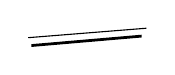
\begin{tikzpicture}\draw (0,0)--(1.5,0.12);\draw[line width=1pt] (0.04,-0.10)--(1.44,0.02);\end{tikzpicture}}

Nous envisageons maintenant une \deleted{gerbe} catégorie de motifs munie d'un \deleted{\unsure{auto}} \unsure{hom} tensoriel dans elle-même qui est ``générateur''. Ainsi $L$ est commutatif et correspond à un groupe \deleted{\unsure{commutatif}} \inserted{\unsure{alg. de type}} \deleted{$\unsure{G}$} multiplicatif $G$, \uline{muni} d'un élément $f$ (``frobenius''), et $G$ est engendré (au sens de Zariski) par $f$. \deleted{Dans le cas qui nous occupe,} \deleted{\unsure{Prenant} \illegible{3} \unsure{donné},}

\deleted{\unsure{soit}}

\mspage{87}

\scanpage{89}
\mspage{88}

\uline{Remarque} 3.13. Voici une généralisation parfois utile de 3.5. b). Considérons une partie $E$ de $X$ telle que pour tout morphisme étale $f:X'\quad X$, $E'=f^{-1}(E)$ soit ``très dense'' dans $X'$ (EGA IV 10.1.3.)\unsure{;} i.e. que pour tout $f$ comme ci-dessus, tout ouvert $U$ de $X'$ qui contient $E'$ soit égal à $X'$. Alors les foncteurs fibres $F_{\bar x}$ sur $X_{\text{ét}}$, pour $x\quad E$, forment déjà une ``famille conservative'' (et par suite les corollaires 3.6., 3.7. et 3.8. restent valables en se bornant à y choisir $x\quad E$). Cela se voit immédiatement en reprenant la démonstration donnée de 3.5. b). Le résultat précédent s'applique notamment dans les siutations suivantes:

a) $X$ est un préschéma de \unsure{Jawobson|Jacobson} (EGA IV 10.4.1.), par exemple localement de type fini sur un corps, ou sur $\operatorname{Spec}(\underline{Z})$, et $E$ est l'ensemble des points fermés de $X$.

b) $X$ est localement de type fini sur un préschéma $S$, et $E$ est l'ensemble des points de $X$ qui sont fermé dans leur fibre.

c) $X$ est localement noethérien, et $E$ est l'ensemble des $x\quad X$ tels que $\bar x$ soit un ensemble fini (i.e. un schéma semi-local de dimension $\quad 1$) cf EGA IV 10.5.3. et 10.5.5.

\scanpage{90}

\diagram{\begin{tikzcd}[row sep=large,cells={nodes={anchor=west}}]
\parbox{.88\linewidth}{a) \deleted{\unsure{protore}} \inserted{groupe de t.m.} $T$ sur $Q$, avec $f\in T(Q)$ engendrant $T$ (Zar)} \arrow[d,Leftrightarrow] \\
\parbox{.88\linewidth}{b) Sous-groupe \deleted{de} $M$ de $\overline Q^*$, stable par $\operatorname{Gal}(\overline Q/Q)$} \arrow[d,phantom,"\unsure{\Downarrow|\Updownarrow}"] \\
\parbox{.88\linewidth}{c) Sous-catégorie \unsure{st. pleine} $\mathcal M'$ de la catégorie des vectoriels sur $Q$ avec endomorphisme \inserted{semi-simple} [i.e. de la catégorie des $Q[X]$ modules \inserted{semi-simples} de dim finie sur $Q$] stable par $\otimes$, $\oplus$, sous objet}
\end{tikzcd}}

\deleted{\unsure{a $\Rightarrow$ b}}
Soit donné un groupe de t.m. $T$, avec ``générateur'' $f\in T(Q)$, et soit donné $G_m\xrightarrow{j}T$, ce qui équivaut à se donner $j^*:M\longrightarrow Z$ \inserted{(invariant par $\operatorname{Gal}(\overline Q/Q)$)}, ou une \unsure{graduation} \inserted{\uline{tensorielle}} sur $\mathcal M$.

\inserted{$\varepsilon:T\longrightarrow G_m$ (\deleted{tel que} $\varepsilon\circ j(\lambda)=\lambda^\alpha$), i.e. $j^*(\unsure{\varepsilon^*})=\alpha$.}
\deleted{\unsure{Soit} $\unsure{j(f)}\unsure{=}\unsure{q}$ \unsure{un élément} \unsure{générateur}}
\inserted{i.e. soit donné un objet $\Lambda$ de $\mathcal M$ \unsure{$W\longrightarrow$} \unsure{de rang 1}}
\deleted{i.e. \illegible{3}}
\inserted{i.e. $\Lambda$ de degré $\alpha$.}
\deleted{\unsure{Posons} $\unsure{\varepsilon^*}=q$ \unsure{et} $|\varepsilon(f)|$}
\margin{\figure{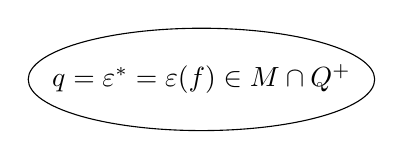
\begin{tikzpicture}\draw (0,0) ellipse (2.2cm and .65cm);\node at (0,0) {$q=\unsure{\varepsilon^*}=\varepsilon(f)\in M\cap Q^+$};\end{tikzpicture}}}

\diagram{\begin{tikzcd}[row sep=large,cells={nodes={anchor=west}}]
\parbox{.88\linewidth}{a) $T^{\unsure{\circ|0}}/\operatorname{Im}j$ est compact.} \arrow[d,Rightarrow] \\
\parbox{.88\linewidth}{b) \inserted{$q>0$ tel} \unsure{que} $\forall\ m\in M$, on a $|m|=\deleted{\unsure{f(f)}}q^{j^*(m)/\alpha}$} \arrow[d,Leftrightarrow] \\
\parbox{.88\linewidth}{c) \inserted{$q>0$ tel} \unsure{que} tout $(E,f)\in\mathcal M$, si $E$ est de degré $i$, les valeurs propres de $f$ dans $E_{\mathbb C}$ sont de val. absolue $q^{i/\alpha}$.}
\end{tikzcd}}

En effet, les valeurs propres de \deleted{$\unsure{E(f)}$ \unsure{et} $f$} $f$, pour $(E,f)\in\mathcal M$ de degré $i$, sont les $m\in M$ avec $\unsure{j(m)}=i$. Donc \deleted{\unsure{b) est plus fort que}} c) et b) sont équivalents.

\deleted{[Ils impliquent a), car $T'=T^{\unsure{\circ|0}}/\operatorname{Im}j$ est un tore \deleted{\unsure{rationnel}} \unsure{possédant} $f'$ ayant la vertu que pour $\forall$ représentation dans un $E$, les valeurs propres de $f'$ opérant sur $E_{\mathbb C}$ sont de val. abs. 1. \unsure{On fera un} \deleted{\unsure{On aura}} \unsure{tore} \unsure{opérant} \inserted{\unsure{semi-simple}} \deleted{\unsure{par des} $\unsure{M^*}$ \unsure{pour} $\unsure{f}$ \unsure{dans} $\operatorname{GL}(E_{\mathbb C})$ \unsure{puis}, \unsure{on le} \unsure{considère} \unsure{opérant} \unsure{sur} $E_{\mathbb C}$ \unsure{et le} \unsure{val. absolue} 1.} Comme $T'_{\mathbb R}$ est un \unsure{sous-groupe} fermé du \unsure{unitaire}, on déduit \unsure{précisément} \illegible{1}]}

\mspage{89}

\scanpage{91}
\mspage{90}
\mspage{43}

supposer $X$ affine et qu'il existe un préschéma affine $X'_1$, de présentation finie, quasi fini et fidèlement plat sur $X$, et un $X$-morphisme $X'_1\longrightarrow X'$, ce qui nous ramène au cas où $f$ est quasi-fini. Quitte à localiser encore sur $X$, au sens de la topologie étale cette fois, on voit qu'il existera un ouvert $X'_1$ de $X'$ tel que $X'_1\longrightarrow X$ soit fini et surjectif, ce qui nous ramène au cas où $f$ est fini et surjectif, déjà traité dans a).

9.4.4. Dans le cas d), on peut supposer (en se localisant sur $X$) que $X$ est réduit à un seul point, et même contenu de 1.1. \unsure{qr'il|qu'il} est spectre d'un corps $k$, puis (quitte à remplacer $X'$ par un ouvert affine non vide) que $X'$ est affine et à fortiori $f$ est quasi compact et quasi séparé. Mais alors il est encore vrai que $f_*$ commute à tout changement de base $Y\longrightarrow X$, comme nous verrons ultérieurement. De plus, $f$ est universellement ouvert (EGA IV 2.4.9.) donc on est sous les conditions de 9.1., et le raisonnement de 9.4.1. s'applique encore.

\margin{\figure{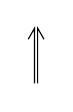
\begin{tikzpicture}\draw (0,0)--(0,0.7)--(-0.08,0.56);\draw (0.04,0)--(0.04,0.7)--(0.12,0.56);\end{tikzpicture}}}

\inserted{Ceci achève la démonstration de 9.4.}

\scanpage{92}

\deleted{\unsure{Il}} Montrons que a) implique c). Soit en effet \deleted{\unsure{donc}} $E$ un vectoriel \deleted{sur $Q$} \inserted{``de degré $i$''} avec $T$ opérant.

\deleted{Alors les \unsure{opér.} \unsure{de} $T_{\mathbb R}$ \unsure{opèrent} sur $E_{\mathbb R}$, et comme}
\deleted{Soit $U$ le plus \unsure{grand sous-groupe}}

Alors $T_{\mathbb R}$ opère sur $E_{\mathbb R}$. Soit $U$ le plus grand sous-tore compact de $T_{\mathbb R}$. Il résulte aisément de l'hyp. a) que $T_{\mathbb R}^{\unsure{\circ|0}}=\unsure{U_{\mathbb R}|U}\cdot S_{\mathbb R}$, où $S=\operatorname{Im}j$, \deleted{et} \inserted{et $U\subset\operatorname{Ker}\varepsilon$.} Donc $f$ est de la forme $uj(x)$, ou du moins il existe un entier \deleted{positif} \inserted{$\nu>0$ tel} que
\[
f^\nu=u\cdot j(x)\qquad u\in U(\mathbb R),\quad x\in\mathbb R^*.
\]
Or $U$ étant compact, les valeurs propres de $\forall$ $u\in U(\mathbb R)$ sont de val. absolue 1, donc celles de $f^\nu$ sont de val. absolue égale à celles de $j(x)$, or $j(x)$ est le \deleted{\unsure{représentation}} \unsure{l'hom.} \unsure{h} par $x^i$, \inserted{d'où les val. propres de $f$ sont de val. abs. $x^{i/\nu}$.} D'autre part \deleted{$\varepsilon(u)=\unsure{0}$} $\varepsilon|U=\unsure{0}$ donc
\[
\varepsilon(f)^\nu=\varepsilon(u)\varepsilon j(x)=\varepsilon j(x)=x^\alpha,
\quad\text{donc}\quad x^{i/\nu}=\varepsilon(f)^{i/\alpha}=q^{i/\alpha},
\]
d'où la conclusion.

\margin{?}
\deleted{N.B. Évidemment b) et c) n'impliquent pas a), \unsure{pour aucun $\alpha$}, car il y a des sous-groupes libres de $Q^*$ de rang $\geq2$ \ldots}

D'autre part, on sait que a équivaut au fait que $\mathcal M$ est (avec ses deux structures suppl. provenant de $j,\varepsilon$) munissable d'une structure ``positive'' du style \unsure{motivique}. Ceci, d'autre part, par un argument connu, implique que

\mspage{91}

\scanpage{93}
\mspage{92}
\mspage{42}

d'où un homomorphisme $f^{\unsure{*}}(G)\longrightarrow F'$ et ce dernier est évidemment compatible avec les données de descente. Il reste à examiner si cet homomorphisme est un \uline{isomorphisme.}

\figure{\begin{tikzpicture}\draw (0,0) .. controls (-0.2,0.15) and (-0.15,0.3) .. (0.1,0.3) -- (4.1,0.48) .. controls (4.35,0.48) and (4.35,0.65) .. (4.2,0.73);\end{tikzpicture}}

Noter que $G$ est aussi définissable par l'exactitude de
\diagram{\begin{tikzcd}G\arrow[r]&f_{\unsure{*}}(F')\arrow[r,shift left=.65ex]\arrow[r,shift right=.65ex]&g_{\unsure{*}}(F'')\end{tikzcd}},
donc pour tout changement de base $Y\xrightarrow{h}X$ \uline{qui commute à la formation de} $f_{\unsure{*}}(F')$ \uline{et} $g_{\unsure{*}}(F'')$, $h^{\unsure{*}}(G)=G_Y$ s'identifie au faisceau ``descendu'' de $F'_{Y'}$ par $Y'\longrightarrow Y$, et bien entendu l'homomorphisme $f_Y^{\unsure{*}}(G_Y)\longrightarrow(F_Y)'$ est celui déduit de $f^{\unsure{*}}(G)\longrightarrow F'$ par changement de base. Or supposons que \uline{le changement de base} $f:Y=X'\longrightarrow X$ \uline{commute à la formation de} $f_{\unsure{*}}(F')$ \uline{et} $g_{\unsure{*}}(F'')$, et notons que comme $Y'=X'\inserted{\times}_X X'$ a une section sur $Y'=X'$, donc $Y'\longrightarrow Y$ est un morphisme de descente \uline{effective} pour toute catégorie fibrée, en particulier pour $\unsure{\mathfrak F|\mathcal F}$, il s'ensuit que $f_Y^{\unsure{*}}(G_Y)\longrightarrow(F_Y)'$ est un isomorphisme, donc $f^{\unsure{*}}(G)\longrightarrow F'$ devient un isomorphisme après changement de base $Y'=X'\quad{}_X X'\longrightarrow X'$. Comme ce dernier à une section, $f^{\unsure{*}}(G)\longrightarrow F'$ est un isomorphisme, donc la donnée de descente envisagée sur $F'$ est effective.

9.4.2. Ceci prouve le théorème 9.4. dans le cas a), grâce à 5.6. Le cas b) résulte également du fait que si $f$ est propre, alors $f_{\unsure{*}}$ commute à \uline{tout} changement de base $Y'\longrightarrow Y$, (qui sera prouvé dans un exposé ultérieur).

9.4.3. Dans le cas c), la question étant locale sur $Y$ on peut

\scanpage{94}

$Q'$: clôture tot. réelle de $Q$ \ldots

\margin{\figure{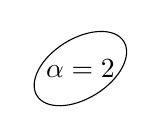
\begin{tikzpicture}\draw[rotate=32] (0,0) ellipse (.65cm and .38cm);\node at (0,0) {$\alpha=2$};\end{tikzpicture}}}

La condition a équivaut à la suivante, si $q\in Q^{*\unsure{+}}$ est $>0$:

\diagram{\begin{tikzcd}[row sep=large,cells={nodes={anchor=west}}]
\parbox{.88\linewidth}{$\left\{\begin{array}{l}\deleted{\unsure{M\subset M}}\ \inserted{\text{Pour tout }\lambda\in M,\ \exists r>0\text{ tel que}}\\\unsure{\lambda}^r\in Q'(i)^*,\quad\text{et pour tout }\lambda\in M,\text{ il existe un}\\\text{entier }i\text{ tel que }|\lambda|=q^{i/2}\quad\text{i.e. }\lambda\bar\lambda=q^i\end{array}\right.$\par\margin{N.B. Le $i$ en question est uniquement déterminé et n'est autre que $j^*(\lambda)$.}} \arrow[d,Leftrightarrow] \\
\parbox{.88\linewidth}{$\left\{\begin{array}{l}\text{Pour tout }\lambda\in M,\ \deleted{\text{il existe}}\ \text{on a }|\lambda|=q^{j^*(\lambda)/2}\quad\text{i.e. }\lambda\bar\lambda=q^{j^*(\lambda)}\end{array}\right.$}
\end{tikzcd}}

\uline{Cor} Soit $\lambda\in\overline Q$, tel que \deleted{il existe $q\in Q^{*+}$, avec}
\figure{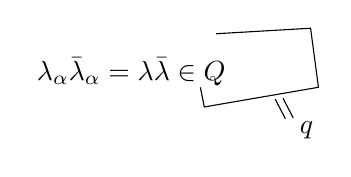
\begin{tikzpicture}
\node[anchor=west] at (0,0) {$\lambda_\alpha\bar\lambda_\alpha=\lambda\bar\lambda\in Q$};
\draw (2.4,.48)--(3.6,.55)--(3.7,-.2)--(2.25,-.45)--(2.2,-.2);
\draw (3.15,-.35)--(3.28,-.6);\draw (3.25,-.34)--(3.38,-.59);
\node at (3.55,-.75) {\inserted{$q$}};
\end{tikzpicture}}
\inserted{$|\lambda_\alpha|^2=|\lambda|^2$}
pour tout conjugué $\lambda_\alpha$ de $\lambda$. Alors $\exists r>0$, tel que $\lambda^r\in Q'(i)$, [donc la condition ne dépend pas des plongements de $\unsure{Q(\lambda)|R(\lambda)}$ dans $\overline Q\subset\mathbb C$], et il existe $M,\varepsilon,j\ldots$ \inserted{relatif à $q$} tel que $\lambda\in M$ (et réciproquement).

\uline{Proposition} Soit $\lambda\in\overline Q^*$, et $q\in Q^{++}$. Conditions équivalentes

(i) $\exists$ entier $i$ tel que pour $\forall$ conjugué $\lambda_\alpha$ de $\lambda$ on ait $|\lambda_\alpha|=q^{i/2}$.
\inserted{i.e. $\lambda_\alpha\bar\lambda_\alpha=q^i$}

\inserted{(\unsure{ii bis}) $\exists$ entier $n>0$ tel que $\lambda^n\in Q'(i)$, et \deleted{\unsure{$\exists$}} entier $i$ tel que $\lambda^n\overline{\lambda^n}=q^{in}$.}

(ii) $\lambda\in Q'(i)$, il existe entier $i$ tel que $|\lambda|=q^{i/2}$ i.e. $\lambda\bar\lambda=q^i$.
\inserted{$|\lambda|=q^{i/2}$, i.e. $\lambda\bar\lambda=q^i$}

(iii) $\exists$ un groupe de t.m. $G$ sur $Q$, et un élément $f$ de $G(Q)$,
\diagram{\begin{tikzcd}G_m\arrow[r,"j"]&G\arrow[r,"\varepsilon"]&G_m\end{tikzcd}},
avec $\varepsilon j(\lambda)=\lambda^2$, \deleted{tel que $\unsure{\operatorname{Ker}\varepsilon}$} \inserted{avec $\operatorname{Ker}\varepsilon$ \uline{compact}}, $\varepsilon(f)=q$, tels que $\lambda$ soit une valeur propre de $f$ pour un $G$-module de dim finie \inserted{sur $Q$} convenable, i.e. $\lambda$ appartient à l'image de l'hom.
\[
M=D(G_{\overline Q})\longrightarrow\overline Q^*
\]
défini par $f$.

(iv) Il existe une algèbre de \unsure{Riemann} \unsure{commutative} sur $Q$ et $f\in A^*$ \inserted{et $i\unsure{\in}\mathbb N$, tels que $ff'=q^i$} et un $Q$-hom. $\unsure{A}\longrightarrow\overline Q$, appliquant $f$ dans $\lambda$.

\mspage{93}
\margin{\uline{N.B.} Si un tel $\lambda$ est réel (donc tot réel!) on a $\lambda^2=q^i$ donc $\lambda=(q^{1/2})^i$, \uline{cas trivial}}

\margin{\deleted{N.B. La condition \uuline{n'implique pas} que $\lambda\in Q'(i)^*$, comme on voit p. ex. en prenant $\lambda=p^{1/4}$; Alors $Q(\lambda)$ n'est ni tot. imaginaire ($Q(p^{1/4})$ est réel) ni tot réel (car il est conjugué à $Q(\sqrt{-\sqrt p})$ qui est \unsure{purement imaginaire}, donc n'est pas $\subset Q'(i)$)}}

\scanpage{95}
\mspage{94}
\margin{-7-}

consequences of 1.9, of which only the following (cf. 1.7) will be stated here, the paper comes to a close.

1.10 Theorem. \uline{Let} $k$ \uline{be a perfect field of} $\dim\leq1$ \uline{and} $G$ \uline{a connected linear group over} $k$. \uline{Then every conjugacy class over} $k$ \uline{contains an element over} $k$.

After the remark that Kneser, using extensions of 1.8, has recently shown (cf. 1.9) that $H^1(k,G)=0$ if $k$ is a p-adic field and $G$ a simply connected semisimple group over $k$, this introduction comes to a close.

\S2. \uline{Some recollections}. In this section we recall some known facts, including some characterizations 2.11 of regular semisimple elements, and establish some notations which are frequently used in the paper. If $k$ is a field, $k^*$ is its multiplicative group. The term ``algebraic group'' is often abbreviated to ``group''. If $G$ is a group, $G_{\unsure{0|O}}$ denotes its identity component. If $x$ is an element of $G$, then $G_x$ denotes the centralizer of $x$ in $G$, and $x_s$ and $x_u$ denote the semisimple and unipotent parts of $x$ when $G$ is linear. Assume now that $G$ is a semisimple group, that is, $G$ is a connected linear group with no nontrivial connected solvable normal subgroup. We write $r$ for the rank of $G$. Assume further that $T$ is a maximal torus in $G$ and that an ordering of the (discrete) character group of $T$ has been chosen. We write $\Sigma$ for the system of roots relative to $T$ and $X_\alpha$ for the subgroup corresponding to the root $\alpha$.

2.1 $X_\alpha$ \uline{is unipotent and isomorphic (as an algebraic group) to the}

\scanpage{96}

\uline{Prop.} Soit $K$ un corps de \unsure{nb} fini sur $Q$, $L$ une extension quadratique de $K$, $p_0$ un idéal premier de $K$, \deleted{$p,p'$} qui se décompose dans $L$ en deux idéaux premiers distincts $p,p'$. Alors il existe un $x\in L^*$ \deleted{dont le diviseur \unsure{doit être}} \deleted{tel que} dont le diviseur soit $h(p-p')$, \inserted{où $h\in N^+$,} et tel que $x\,{}^\sigma x=1$, où $\sigma$ est l'autom. non trivial de $L/K$.

\margin{Plus précisément à torsion près, les diviseurs des \deleted{\unsure{nb}} éléments de $L$ tels que $N_{L/K}x=1$, \deleted{\unsure{$N_{L/K}$}} sont les diviseurs de $L$ de norme $1$!}

En effet, \deleted{comme le groupe des} si $h$ est l'ordre du groupe de classes \inserted{de div.} de $L$, il existe un $y$ de diviseur $h(p-p')$. Alors $y\,{}^\sigma y$ est un élément de $K$ dont le diviseur est évidemment nul, donc c'est une unité $u$.
Donc si $z=y^2$, alors \deleted{$\unsure{x\bar x}\quad\unsure{x\,{}^\sigma x}$} $z\cdot{}^\sigma z=(y\cdot{}^\sigma y)^2=u^2$, donc si $x=\dfrac{z}{u}=\dfrac{y^2}{Ny}$, on aura
\[
\operatorname{div}x=\operatorname{div}z=2\operatorname{div}y=2h(p-p'),\qquad\text{et}\qquad x\,{}^\sigma x=(z\,{}^\sigma z)/u^2=1.
\]

\uline{N.B.} Supposons que $K$ est tot. réel \deleted{\unsure{galoisienne de $Q$}}, \deleted{et $L$ une \unsure{ext.}} \inserted{$L$ \deleted{\unsure{ext.}} qu. de $K$; supposée \uline{galoisienne} sur $Q$,} \deleted{\unsure{et $L$}} tot. imaginaire. Soit $p$ un nb premier, et $p_0$ idéal de $K$ au dessus de $p$, supposons qu'il n'y ait qu'un \uline{seul idéal} \inserted{premier} $p$ \deleted{\unsure{de}} de $L$ sur $K$. Soit $\lambda$ un \uline{entier} de $L$ tel que $\lambda\bar\lambda=p^i$. Alors $\lambda^2\bar\lambda^2=p^{2i}$ donc si $\mu=\lambda^2/p^i=\dfrac{\lambda^2}{N_{L/K}\lambda}$ on aura $\mu\bar\mu=1$, \deleted{et $\mu$ est une unité} qui implique que $\mu$ est une unité en $p$, donc ($K$ est galoisien) pour $\forall$ idéal premier au dessus de $p$ \unsure{par $Q$-conjugaison|puisque $\mu=\bar\mu^{-1}$} (l'hyp. sur $p_0$ \unsure{se transpose aux $p_0$ conj.}) donc $\mu$ est une unité. (NB. $\lambda$ \unsure{aux $p$|aussi} est une unité \unsure{exc. $p$}.) donc une racine de l'unité. Donc $\lambda=p^{i/2}u$, $u$ racine de l'unité!

\mspage{95}

\scanpage{97}
\margin{-5-}

for $L$, but there does not seem to be any simple way of relating 1.4 and 1.5 to their analogues for $L$.

We now introduce a perfect subfield $k$ of $K$, although it appears from recent results of A. Grothendieck on semisimple groups over arbitrary fields that the assumption of perfectness is unnecessary for most of what follows.

1.6 Theorem. \uline{Let} $G$ \uline{be over} $k$, \uline{and assume either that} $G$ \uline{splits over} $k$ \uline{or that} $G$ \uline{contains a Borel subgroup over} $k$ \uline{but no component of type} $A_n$ ($n$ \uline{even}). \uline{Then the set} $N$ \uline{of} 1.4 \uline{can be constructed over} $k$ (\uline{by appropriate choice of} $T$, $\sigma_i$, \uline{etc.}).

Together with 1.4 this implies that if $G$ is simply connected in 1.6 the natural map from the set of regular elements over $k$ to the set of regular classes over $k$ is surjective. For a group of type $A_n$ ($n$ even) we have a substitute (see 9.7) for 1.6 which enables us to show:

1.7 Theorem. \uline{Assume that} $G$ \uline{is simply connected and over} $k$ \uline{and that} $G$ \uline{contains a Borel subgroup over} $k$. \uline{Then the natural map from the set of semisimple elements over} $k$ \uline{to the set of semisimple classes over} $k$ \uline{is surjective. In other words, each semisimple class over} $k$ \uline{contains an element over} $k$.

Theorems 1.6 and 1.7 are proved in \S9 where it is also shown (see 9.1 and 9.10) that the assumption that $G$ contains a Borel subgroup over $k$ is essential.

\mspage{96}

\scanpage{98}

Soit $K$ une extension \deleted{\unsure{gal.}} \deleted{tot.} réelle finie de $Q$, $L$ ext. quadratique tot. imaginaire de $K$, $q=p^{\unsure{r}}$ une puissance de nb premier. On cherche les $\lambda\in K$ \uline{entiers} tels que $\lambda\bar\lambda=q^i$, i.e. $|\lambda|=q^{i/2}$, \inserted{pour $i$ convenable $\in N$.} Ce sont des unités exc. $p$, et ils engendrent \deleted{le groupe des} un sous-groupe du groupe \deleted{\unsure{U des} unités exc. $p$, \unsure{tel le $\lambda$ est}} formé des $\unsure{\lambda'|\lambda}$ unités exc. $p$ tels que $\lambda\bar\lambda=q^i$ ($i\in Z$). Notons que \deleted{ce sont des unités \uline{absolues} exc. $p$. Donc \unsure{finalement il suffit en $\lambda$ d'écrire} $p^{i/2}u$, avec $u$} si $q$ est un carré de $K$, on peut écrire les $\lambda$ sous la forme $\lambda=q^{i/2}u$, où $u$ est une unité exc. $p$ telle que $u\bar u=1$, ce qui implique que $u$ est une \uline{unité absolue} exc. $p$. Les $u$ forment un groupe $U$, et l'hom
\[
U\unsure{\text{—}|\longrightarrow} Z^P\qquad u\unsure{\sim|\longmapsto}(v_{\mathfrak p}(u))_{\mathfrak p\in P}
\]
(où $P$ désigne l'ens des $\mathfrak p$ de $L$ sur $p$) est de noyau fini. D'après la prop. plus haut, son image est \inserted{contenue et} d'indice fini dans $(Z^{\unsure{P}})'$, \deleted{$P'$ est l'ens des $\mathfrak p$} formé des diviseurs de trace \inserted{rel. à $K$} nulle. Donc si pour $\forall$ $p_0$ \deleted{\unsure{de $K$}} idéal premier de $K$ sur $p$ qui \uline{splitte en deux} dans $L$, on choisit un $\mathfrak p$ au dessus, on trouve un isom. mod. groupes finis $U\simeq Z^Q$, $Q$ est l'ens des $p_0$

\mspage{97}

\scanpage{99}
\margin{-4-}

\uline{of regular classes of} $G$.

In 7.4 an example of $N$ is given: in case $G$ is of type $\mathrm{SL}(r+1)$ we obtain one of the classical normal forms under conjugacy. This special case suggests the problem of extending the normal form $N$ from regular elements to arbitrary elements. In 7.1 it is shown that $N$ is a closed irreducible subset of $G$, isomorphic as a variety to affine $r$-space $V$, and in 7.9 (this is the main lemma concerning $N$) that if $G$ is simply connected and $\chi_i$ ($1\leq i\leq r$) denote the fundamental characters of $G$ then the map $x\to(\chi_1(x),\chi_2(x),\ldots,\chi_r(x))$ induces an isomorphism of $N$ on $V$. Then in \S8 the proof of 1.4 is given and simultaneously the following important criterion for regularity is obtained.

1.5 Theorem. \uline{If} $G$ \uline{is simply connected, the element} $x$ \uline{is regular if and only if the differentials} $d\chi_i$ \uline{are independent at} $x$.

At this point some words about recent work of B. Kostant are in order. In [3] and [4] he has proved, among other thing, the analogues of our above discussed results that are obtained by replacing the semisimple group $G$ by a semisimple Lie algebra $L$ over the complex field (any algebraically closed field of characteristic $0$ will serve as well) and the characters $\chi_i$ of $G$ by the basic polynomial invariants $u_i$ of $L$. The $\chi_i$ turn out to be considerably more tractable than the $u_i$. Thus the proofs for $G$ with no restriction on the characteristic are simpler than those for $L$ in characteristic $0$. Assuming both $G$ and $L$ are in characteristic $0$, substantial parts of 1.1, 1.2, and 1.3 can be derived from their analogues

\mspage{98}

\scanpage{100}

Conditions nécessaires pour qu'un $\lambda\in\bar Q$ soit valeur propre d'un \unsure{frobénius}, pour une variété projective lisse définie sur le corps $\mathbb F_q$, $q=p^n$:

\deleted{1) $\lambda\in Q'(i)$

2) \deleted{\unsure{$\lambda$}} $\lambda^2$ est de la forme $q^iu$, où $u\in Q'(i)$ est une unité exc. $p$.

Si $\mathfrak p,\mathfrak p'$ sont deux idéaux premiers de}

1) \fbox{$\lambda$ entier algébrique}

2) \fbox{$\lambda\in Q'(\sqrt{-1})$}

3) $\lambda^{\unsure{2}}=q^{i/2}u$, \inserted{$i\in Z$,} avec $u$ une unité \inserted{absolue} exc. $p$ (cela détermine évidemment de façon unique $i$ et $u$)

\inserted{\fbox{$\exists i$ tel que $|\lambda_\alpha|=q^{i/2}$ pour \unsure{tt|$\forall$} conjugué $\lambda_\alpha$} !}

\margin{N.B. $q^{i/2}\in Q'$!}

\margin{\uline{N.B.} Les conditions 2) 3) 4) sont ``\unsure{linéaires}'', la condition 1) est seulement \unsure{additive} ... On désigne par $M(q^{\unsure{n}})$ le groupe de $Q'(i)^*$ défini par \deleted{\unsure{2)}} 3) 4).}

\deleted{4) Si $\mathfrak p,\mathfrak p'$ sont deux idéaux premiers de $Q'(\sqrt{-1})$ au dessus du même idéal premier de $Q'$, on a
\figure{\begin{tikzpicture}[x=1cm,y=1cm]
\node at (0,1.5) {$v_{\mathfrak p}(u)+v_{\mathfrak p'}(u)=0$};
\node at (3.4,1.5) {i.e.};
\node[draw,rectangle] (f) at (7,1.5) {$v_{\mathfrak p}(\lambda)+v_{\mathfrak p'}(\unsure{\lambda^*|\lambda})=\dfrac{in}{2}$};
\node[align=center] at (7,0) {$v_{\mathfrak p}$ normalisés tels que\\$v_{\mathfrak p}(p)=1$.};
\node[draw,ellipse,align=center] (c) at (2,-.4) {Conséquence\\de \uline{2 et 3}\\!!!};
\draw[->,double] (c.north east) -- (f.south west);
\end{tikzpicture}}}

L'entier $i$ qui intervient ici est appelé le \uline{poids} de $\lambda$ (relativement à $q=p^n$). \deleted{\unsure{Le fait que le poids est}} Si les conditions \deleted{\unsure{est donc}} analogues sont satisfaites pour $q'=p^m$, elles le sont pour $q$, et le poids $i$ rel. à $q$ est égal à $mi'$, où $i'$ est le poids par rapport à $q'$.

\margin{\unsure{Th. d'existence en $\mathrm{Fr}$ sur $\mathbb F_q$}}

\margin{\figure{\begin{tikzpicture}\draw (0,0)--(0,1.1);\draw (.06,0)--(.06,1.1);\draw (1.35,0)--(1.35,1.15);\end{tikzpicture}}}

\uline{Conjecture} \deleted{\unsure{est elle}} \uline{forte} \uline{Les conditions nécessaires précédentes sont suffisantes}

Cela déterminerait donc explicitement, en termes arithmétiques simples, le groupe de Galois motivique \inserted{$G$} sur $\mathbb F_q$. Vérifions que cela donne bien

\mspage{99}

\scanpage{101}
\margin{96}

\begin{center}
Chapter III

Some Applications of the Criterion of Projectivity

of Abstract Complete Varieties.
\end{center}

In this chapter we will examine some of the applications of the following assertion which follows from theorem 2:

\uline{Let} $V$ \uline{be a nonsingular complete algebraic variety} $\dim V=s$ \uline{and} $D$ \uline{be a divisor on} $V$ \uline{such that} $D^kW_k>0$ \uline{for any irreducible subvariety} $W_k$ \uline{of dimension} $k$, $k=\overline{1,s}$ ($D^sV=D^s$). \uline{Then, at sufficiently large} $n$, \uline{the mapping of the variety} $V$ \uline{into a projective space, corresponding to the fibre} $[nD]$, \uline{becomes a biregular imbedding}.

Let $V$ be a complete normal algebraic variety, $\dim V=s$ and $U$ be an open set on $V$, being a quasi-projective variety (that is, allowing realization in the form of an open subset of a projective algebraic variety).
\margin{p. 218}
Let $x_0,x_1,\ldots$ be homogeneous coordinates, corresponding to $U$, $x_0\ne0$, and $F_j=\dfrac{x_j}{x_0}$. Let $\unsure{\{F\}|[F]}$ be \deleted{a}\inserted{\unsure{the}} linear space over $k$, generated by the functions $F_j$, and $\{T_{\inserted{\ell}}\}$ be a totality of irreducible $s-1$ dimensional components of the set $V-U$,
\margin{$\ell$}
\[
\tau_\ell=\min_j n_{T_\ell}(F_j)
\]
where $n_{T_l}(F_j)$ denotes the order of the function $F_j$ on the divisor $T_l$. Let a function $\varphi\in\unsure{\{F\}|[F]}$ be such that,

\mspage{100}

\scanpage{102}

le \unsure{schéma|résultat} correct pour le $G/G^{\unsure{\circ|0}}$: car en effet, il est dual au groupe des racines de l'unité, or ce dernier est bien le dual de $\widehat Z$!

\margin{\[
M(q^m)\subset M(\underset{\shortparallel\,p^n}{q})\subset M(p)
\]
\[
M(q^m)^m\subset M(q)^m\subset M(q^m)\subset M(q)
\]}

Soit $M(q)$ le s-gr. de $Q'(i)^*$ qu'on définit en termes de $q$ ci-dessus, soit \deleted{$\unsure{T}$} $\inserted{f_q\in}G(q)$ son dual, qui est le groupe de Galois motivique sur $\mathbb F_q$. Considérons l'extension $\mathbb F_{q^m}$ de $\mathbb F_q$, d'où
\deleted{$\unsure{G_q^m}$}
\diagram{\begin{tikzcd}[column sep=large]
G(q)&G(q^m)\arrow[l]\\
(f_q)^m&f_{q^m}\arrow[l,rightsquigarrow]
\end{tikzcd}}

\margin{$M(q)\simeq Z\times M^{\unsure{\circ|0}}\deleted{(q)}$ si $q=p^{\unsure{n}}$, \unsure{$n$ pair}. $M^{\unsure{\circ|0}}\deleted{(q)}$ formé des $u\in Q'(i)^*$ qui sont des unités abs. exc. $p$, et vérifient $v_{\mathfrak p}(u)+v_{\mathfrak p'}(u)=0$; le premier facteur \deleted{\unsure{$Z$}} $Z$ correspond à $q^{1/2}$. \unsure{Les homomorphismes de transition entre les} $M(q)$ \unsure{sont} l'identité sur le facteur $Z$, et la multiplication par $m$ sur le facteur $M^{\unsure{\circ|0}}$.}

\deleted{\unsure{de fait}} on voit que l'hom désigné \unsure{$\alpha$} est induit par
\diagram{\begin{tikzcd}[column sep=huge]
M(q)\arrow[r,"{\text{élévation à la puissance }m}"]&M(q^m)
\end{tikzcd}}
dont le noyau est comme de juste \deleted{$\unsure{Z}$} $\mu_m$ (dual de $Z/mZ$) et dont l'image est $M(q)^m$ donc contient $M(q^m)^m$, dont le conoyau est annulé par $m$. Par suite, le \deleted{conoyau} noyau de $\alpha$ est annulé par $m$.

\deleted{\unsure{Comme}} Considérons la limite inductive des $M(q)$ ($q$ variant multiplicativemt) par les hom précédents: on trouve $M(p^\infty)$, un groupe sans torsion dont le dual doit être le groupe de

\mspage{101}

\scanpage{103}
\margin{IV.8}

$\psi^*\psi_*(\mathcal A')$ to $\mathcal A'$ corresponding to the identity homomorphism on $\psi_*(\mathcal A')$. We denote this map by $\sigma_{\mathcal A'}:\psi^*\psi_*(\mathcal A')\to\mathcal A'$. If $\mathcal A$ is a sheaf of rings on $X$, there is a canonical ring homomorphism from $\mathcal A$ to $\psi_*\psi^*(\mathcal A)$ corresponding to the identity homomorphism on $\psi^*(\mathcal A)$. We denote this map by $\rho_{\mathcal A}:\to\psi_*\psi^*(\mathcal A)$.

Now suppose $\Psi:(Y,\mathcal A')\to(X,\mathcal A)$ is a map of ringed spaces; i.e. $\Psi=(\psi,\theta)$ where $\psi$ is a continuous map from $Y$ to $X$ and $\theta$ is a homomorphism of sheaves of rings $\theta:\mathcal A\to\psi_*(\mathcal A')$. Then for any $\mathcal A'$-module $\mathcal M'$, $\psi_*(\mathcal M')$ can be made into an $\mathcal A$-module by means of the operation of $\theta$. When $\psi_*(\mathcal M')$ is considered a module over $\mathcal A$ in this way, it is denoted $\Psi_*(\mathcal M')$. We have the following canonical functorial homomorphisms [8, 0; \S\ 4.2]:
\[
h_*:\Psi_*(\uline{\mathrm{Hom}}_{\mathcal A'}(\mathcal M',\mathcal N'))\longrightarrow\uline{\mathrm{Hom}}_{\mathcal A}(\Psi_*(\mathcal M'),\Psi_*(\mathcal N'))
\]
\[
t_*:\Psi_*(\mathcal M')\underset{\mathcal A}{\otimes}\Psi_*(\mathcal N')\longrightarrow\Psi_*(\mathcal M'\underset{\mathcal A'}{\otimes}\mathcal N').
\]

On the other hand we have the map $\psi^*(\theta):\psi^*(\mathcal A)\to\psi^*\psi_*(\mathcal A')$, and so we have $\sigma_{\mathcal A'}:\psi^*(\theta):\psi^*(\mathcal A)\to\mathcal A'$. $\mathcal A'$ is an algebra over $\psi^*(\mathcal A)$ by the means of this map, and if $\mathcal M$ is an $\mathcal A$-module, we define the $\mathcal A'$-module $\Psi^*(\mathcal M)$ to be $\psi^*(\mathcal M)\underset{\psi^*(\mathcal A)}{\otimes}\mathcal A'$.

There is a canonical functorial isomorphism [8, 0; 4.33.1]
\[
t^*:\Psi^*(\mathcal M)\underset{\mathcal A'}{\otimes}\Psi^*(\mathcal N)\quad\Psi^*(\mathcal M\underset{\mathcal A}{\otimes}\mathcal N).
\]

It can be shown that there is a natural isomorphism from $\mathrm{Hom}_{\mathcal A'}(\Psi^*(\mathcal M),\mathcal M')$ to $\mathrm{Hom}_{\mathcal A'}(\mathcal M,\Psi_*(\mathcal M'))$ for all $\mathcal A$-modules $\mathcal M$ and $\mathcal A'$-modules $\mathcal M'$. By means of this isomorphism we can define the $\mathcal A$-homomorphism $\rho_{\mathcal M}:\mathcal M\to\Psi_*\Psi^*(\mathcal M)$ and the $\mathcal A'$-homomorphism

\mspage{102}

\scanpage{104}

Galois motivique de $\overline{\mathbb F}_p$. \deleted{\unsure{Comme les} $M^{\unsure{\circ|0}}(q^{\unsure{m}})\quad M^{\unsure{\circ|0}}(q)$ \unsure{induisent un isom.}
\[
M^{\unsure{\circ|0}}(q')\otimes_ZQ\quad M^{\unsure{\circ|0}}(q)\otimes_ZQ,
\]}
on constate que $M^{\unsure{\circ|0}}(q^\infty)$ \deleted{que} s'identifie à \deleted{\unsure{un sous-groupe}} de $M^{\unsure{\circ|0}}\deleted{(\unsure{q})}\otimes_ZQ$, qui est lui-même isomorphe au quotient $P/U$, $U$ étant le groupe des racines de l'1, et $P$ étant le sous-groupe de $\bar Q^*$ formé des $\lambda$ tels que $\lambda^n\in M^{\unsure{\circ|0}}\deleted{(\unsure{q})}$ pour $n$ assez grand.

\margin{On aura $M(q^\infty)\simeq Z\times M^{\unsure{\circ|0}}(q^\infty)$, $M^{\unsure{\circ|0}}(q^\infty)=\varinjlim M^{\unsure{\circ|0}}(q^n)\simeq M^{\unsure{\circ|0}}\otimes_ZQ$.}

\deleted{L'hom
\diagram{\begin{tikzcd}[column sep=large]
M^{\unsure{\circ|0}}(q^{\deleted{\unsure{m}}}=p^n)\arrow[r]&P/U
\end{tikzcd}}
s'obtient par
\[
\lambda\longrightarrow\lambda^{1/n}\bmod U
\]
(où la détermination de $\unsure{U|\lambda^{1/n}}$ qu'on prend est sans importance). On a bien
\[
(\lambda^{1/n})^{\unsure{na}}=\lambda^{\unsure{a}}\in M^{\unsure{\circ|0}}(p^n)
\]
\inserted{$M^{\unsure{a|\circ}}(p)$}
car $M(p^n)^{\unsure{a}}\subset M(p)$. Trouve-t-on $P^{\unsure{\circ|0}}/U$ tout entier? \deleted{\unsure{On peut}} \inserted{Si} $\lambda\in\bar Q^*$ tels que $\lambda^n\in M^{\unsure{\circ|0}}(p)$, \deleted{\unsure{donc si}} provient-il du $\mu\in M^{\unsure{\circ|0}}(p^m)$, i.e. \deleted{\unsure{est il de}} a-t-on $\lambda^m\in M^{\unsure{\circ|0}}(p^m)$ pour $m$ convenable??

On peut \deleted{\unsure{supposer de $\lambda$ s'exprime}} se borner aux $m=nh$ multiples de $n$, et la question devient si pour $\forall$ $\lambda\in M^{\unsure{\circ|0}}(p)$, $n\deleted{\unsure{h}}\in N^*$ étant donnés, il existe un $h\in N^*$ tels que $\lambda^h\in M^{\unsure{\circ|0}}(p^{hn})$.}

\mspage{103}

\scanpage{105}
\margin{94}

be a basis of the group $H^0(V,O_V[N\widetilde H])$. We have:
\[
f_*(O_V[N\widetilde H])\simeq(f_*O_V)[NH]_{\bar V}.
\]

From the isomorphism of ringed spaces $(V,f^*O_{\bar V})$ and $(\bar V,O_{\bar V})$ we obtain the isomorphism of the sheaves $O_V[N\widetilde H]$ and $(f_*O_V)[NH]_{\bar V}$.

Let $\bar\alpha,\bar y,\bar y_1,\ldots,\bar y_M$ be the elements over $\bar V$, corresponding to the elements $\alpha,y,y_1,\ldots,y_M$. Since $\alpha y\in O_V[N\widetilde H](P)$, then
\[
\bar\alpha\bar y\in(f_*O_V)[NH]_{\bar V}(\bar P).
\]

According to the definition of the number $N$, there exist $\beta_\nu\in O_{\bar V,\bar P}$ such that
\[
\bar\alpha\bar y=\sum_{\nu=1}^M\beta_\nu\bar y_\nu
\]

Hence, if we denote by the same symbol the functions, corresponding to $\beta_\nu$ at the mapping $f$, we obtain:
\[
\alpha y=\sum_{\nu=1}^M\beta_\nu y_\nu
\]
or, since $y\ne0$ in $P$
\[
\alpha=\sum_{\nu=1}^M\beta_\nu\frac{y_\nu}{y}.\tag{24}
\]

\mspage{104}

\scanpage{106}

La forme plus faible, ``géométrique'' de la conjecture ci-dessus dirait que \deleted{\unsure{c'est}} l'on obtient bien ainsi, par le schéma associé à $M^{\unsure{\circ|0}}\otimes_ZQ$ (sur lequel $\pi$ opère ...), la \deleted{\unsure{groupe de}} ``partie compacte'' du \deleted{\unsure{son}} groupe de Galois motivique de $\overline{\mathbb F}_p$, qui serait donc isom. à
\[
G\simeq\uline{D}(\unsure{M_0|M^{\unsure{\circ|0}}}\otimes Q)\times G_m
\]
avec l'hom inj: $G_m\longrightarrow G$ s'identifiant à $j$, et \deleted{$\unsure{G_m}$} $(x,\lambda)\unsure{\text{—}|\longrightarrow}\lambda^2$ s'identifie à $\varepsilon$.

En termes de valeurs propres de Frobenius:

\margin{\figure{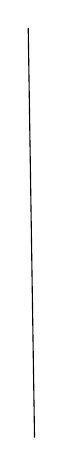
\begin{tikzpicture}\draw (0,0)--(-.08,5.2);\end{tikzpicture}}}

\uline{Conjecture faible} \unsure{Les|Soit} $\lambda\in\bar Q^*$, \deleted{\unsure{tel qu'il}\inserted{\deleted{\unsure{tel}}} \unsure{existe un entier $n>0$ avec $\lambda^n$ satisfaisant aux conditions, de la forme $p$}} un \uline{entier} algébrique, \deleted{tel qu'il existe un entier} tel qu'il existe un entier $i\geq0$, de sorte que $\lambda=p^{i/2}u$, \deleted{\unsure{soit un}} où $u$ est une \uline{unité absolue} \uline{exc.} $p$, et qu'il existe un entier $n>0$ tel que $u^n\in Q'(i)^*$, et $v_{\mathfrak p}(u^n)+v_{\mathfrak p'}(u^n)=0$ pour $\forall$ couple d'idéaux premiers de $Q'(i)$ induisant le même idéal premier de $Q'$. Alors il existe un entier $m>0$ tel que $\lambda^m=(p^m)^{i/2}u^m$ soit \inserted{une} valeur propre de frobenius \unsure{$f_{q^m}$} dans un motif semi-simple \inserted{de poids $i$} convenable sur $\mathbb F_{q^m}$

\margin{Résulte \unsure{probablement} de la théorie des multiplications complexes: cf. \uline{Taniyama--Shimura}}

\mspage{105}

\scanpage{107}
\margin{92}

$H^0(V,O_V[nD])$. Let us examine a covering $\{U_\mu\}$ of the variety $V$, where $U_\mu$ is an addition to the variety of zeros of the cross-section $\psi_\mu$, $\mu=\overline{1,R}$.

Since $\psi_\mu$ do not have common zero, then $\{U_\mu\}$ covers all $V$. Some hyperplane cross-section $H_\mu$ of the variety $\bar V$ becomes the image of the variety of zeros of the cross-section $\psi_\mu$ at the mapping $f$. The family $\{U_\mu\}$, where $\bar U_\mu=fU_\mu$, forms an open covering of the variety $\bar V$. The fibre $[H]_{\bar V}$ is defined for this covering by the transition function:
\[
\bar R_{\mu_1,\mu_2}=\frac{\psi_{\mu_2}}{\psi_{\mu_1}}\quad\text{in }U_{\mu_1}\cap U_{\mu_2}
\]

Consider a covering $\{U_{i\mu}\}$ of the variety $V$, where
\[
U_{i\mu}=U^{(i)}\cap U_\mu
\]
($\{U^{(i)}\}$ is the covering of $V$, in which $[D]$ was defined originally). For $\{U_{i\mu}\}$, $[nD]$ is defined by the transition functions:
\[
{}_1R_{i_1\mu_1,i_2\mu_2}=R^n_{i_1i_2}\quad\text{in }U_{i_1\mu_1}\cap U_{i_2\mu_2}
\]
($R_{ij}$ are the transition functions for $[D]$ and $\{U^{(i)}\}$); $[\widetilde H]$ is defined for $\{U_{i\mu}\}$ by the transition functions:
\[
{}_2R_{i_1\mu_1,i_2\mu_2}=\frac{\psi_{\mu_2}}{\psi_{\mu_1}}=\frac{\psi^{(\unsure{i_1|i_2})}_{\mu_2}}{\psi^{(i_1)}_{\mu_1}}\quad\text{in }U_{i_1\mu_1}\cap U_{i_2\mu_2}
\]

\mspage{106}

\scanpage{108}

$K$ extension tot. réelle \margin{[i.e. si $K$ défini par $H\subset\pi_1(Q)$, $H$ ne contient aucun conjugué de $\tau$, $\tau$ la conjugaison ordinaire)}

A) $L$ extension quadratique, $L=K(\unsure{x|z})$, $x^2+ax+b=0$ ($a,b\in K$).
\inserted{$\sigma$ l'élément non trivial de $\operatorname{Gal}(L/K)$, donc $\sigma x=\bar x$ pour $\forall$ $x$}
\margin{$a=x+{}^\sigma x$, $b=x\,{}^\sigma x$}
Conditions équivalentes:
\diagram{\begin{tikzcd}[row sep=large]
\text{$L$ tot. imaginaire}\arrow[d,phantom,"\unsure{\Updownarrow|\Downarrow}"]\\
\begin{gathered}\text{Pour $\forall$ plongt de $K$ dans $R$, }\Delta=\unsure{a^2}-4b\\=(x-{}^\sigma x)^2\text{ est }\unsure{<}0,\text{ i.e. $\Delta$ est}\\\text{tot. \deleted{positif} négatif}\end{gathered}\\
\deleted{\begin{gathered}\text{$L$ est stable par }\lambda\mapsto\bar\lambda,\text{ et}\\(x-\bar x)^2\text{ est tot. positif}\end{gathered}}\arrow[u,Leftrightarrow]
\end{tikzcd}}
\deleted{Alors $\sigma$ est la conj. \unsure{complexe}.}

B) Soit $x\in\bar Q\subset C$. Conditions équivalentes
\diagram{\begin{tikzcd}[row sep=large]
\begin{gathered}1)\quad\left\{\begin{aligned}&x+\bar x\ [\text{et }x\bar x\text{ sont}]\ \text{tot. réels}\\&(x-\bar x)^2\text{ est tot. \deleted{\unsure{positif} \unsure{$\leq0$}} négatif}\end{aligned}\right.\end{gathered}\arrow[d,Leftrightarrow]\\
\begin{gathered}2)\quad\deleted{x\text{ est }\unsure{\text{un}}}\ \exists\text{ un $K$ tot. réel et une}\\\text{extension $L$ tot. imaginaire de $K$, dont}\\\text{$x$ soit un générateur.}\end{gathered}\arrow[d,Leftrightarrow]\\
2')\quad\deleted{\unsure{x}}\ x\in Q'(i)-Q',\quad\text{i.e.}
\end{tikzcd}}
\inserted{conséquence des autres, car $x\bar x=\frac14[(x+\bar x)^2-(x-\bar x)^2]$}

En effet, $2)\Rightarrow1)$ en vertu de A), et pour $1)\Rightarrow2)$ il suffit de prendre $K=Q(a,b)$ où $a=x+\bar x$, $b=x\bar x$, et appliquer encore A). \uline{Remarque} Cet \unsure{ensemble par les} conditions de 1) est stable par conjugaison, ce qui n'était pas évident autrement.

\deleted{3) $x\bar x$ est tot. str. positif et de même pour $x_\alpha\bar x_\alpha$ pour $\forall$ conjugué de $x$}

C) Soit $x\in\bar Q\subset C$. Conditions équivalentes
\diagram{\begin{tikzcd}[row sep=large]
\begin{gathered}1)\quad x+\bar x\text{ tot. réel,}\quad(x-\bar x)^2\text{ tot. négatif}\end{gathered}\arrow[d,Leftrightarrow]\\
2)\quad\exists K,L\text{ comme plus haut,}\quad x\in\deleted{\unsure{K}}L\arrow[d,Leftrightarrow]\\
3)\quad x\in Q'(i).\arrow[d,Rightarrow,bend right=45]\\
\begin{gathered}\unsure{4)}\quad x\bar x\text{ tot. positif,}\quad\deleted{\unsure{\text{et de même}}}\ \inserted{\text{ainsi que}}\\x_\alpha\bar x_\alpha\text{ pour $\forall$ conjugué $x_\alpha$ de $x$.}\end{gathered}
\end{tikzcd}}
\deleted{\unsure{après}}
\margin{\unsure{2}\ $\Uparrow$}

\mspage{107.}

\scanpage{109}
\margin{-10-}

$G_{x\unsure{0|O}}$, \uline{the intersection} $G'\cap T'$ \uline{finite, and} $\operatorname{rank}G'+\operatorname{rank}T'=r$. \uline{Further} $G'$ \uline{and} $T'$ \uline{are uniquely determined as the commutator subgroup and the identity component of the centre of} $G_{x\unsure{0|O}}$. (b) \uline{The unipotent elements of} $G_x$ \uline{are all in} $G'$.

Part (b) follows from (a) because $G_{x\unsure{0|O}}$ contains the unipotent elements of $G_x$ by [8, p. 6-15, Cor. 2]. For the proof of (a) we may imbed $x$ in a maximal torus $T$ and use the above notation. If $y$ in $G_x$ is written $y=u\sigma_wb$ as in 2.4 then the uniqueness in 2.4 implies that $u,\sigma_w$ and $b$ are in $G_x$. By 2.1 and 2.2 we get:

2.8 $G_x$ \uline{is generated by} $T$, \uline{those} $X_\alpha$ \uline{for which} $\alpha(x)=1$, \uline{and those} $\sigma_w$ \uline{for which} $wx=x$. Then $G_{x\unsure{0|O}}$ is generated by $T$ and the $X_\alpha$ alone because the group so generated is connected and of finite index in $G_x$ (see [8, p. 3-01, Th. 1]). Let $G'$ be the group generated by the $X_\alpha$ alone, and let $T'$ be the identity component of the intersection of the kernels of the roots $\alpha$ such that $\alpha(x)=1$. Then $G'$ is semisimple by [8, p. 17-02, Th. 1], and the other assertions of (a) are soon verified.

2.9 Corollary. \uline{In} 2.7 \uline{every maximal torus containing} $x$ \uline{also contains} $T'$.

For in the above proof $T$ was chosen as an arbitrary torus containing $x$.

2.10 \uline{Remark}. That $G_x$ in 2.7 need not be connected, even if $x$ is regular, is shown by the example: $G=\mathrm{PSL}(2)$, $x=\operatorname{diag}(i,-i)$, $i^2=-1$.

\mspage{108}

\scanpage{110}
\margin{\diagram{\begin{tikzcd}[row sep=small,column sep=small]
& & \deleted{\unsure{Q'(i)}}\arrow[dl] & \\
Q'(i) \arrow[r,dash] \arrow[d,dash] & L \arrow[d,dash] \arrow[dr,dash] & & \arrow[ddd,phantom,"{\left.\begin{matrix}\vphantom{L}\\\vphantom{L_0}\\\vphantom{K_0}\\\vphantom{Q}\end{matrix}\right)\unsure{\text{galoisienne}}}"] \\
Q' \arrow[r,dash] & K \arrow[dd,dash] \arrow[dr,dash] & L_0 \arrow[d,dash] & \\
& & K_0 & \\
& Q & &
\end{tikzcd}}}

On veut construire le groupe de t.m. \inserted{$G(q)$} associé à l'ens $M(q)$ des $\lambda\in L$ tels que $\lambda\bar\lambda=q^i$, et $\lambda$ unités exc. $p$. On a vu que
\[
M_0(q)/\text{Torsion}\subset (\mathbb Z^P)' \qquad (1)
\]
\margin{N.B. $M_0(q)$ \inserted{$=M_0(p)$} \unsure{gr. des} unités $u\in L$ \unsure{qui sont} exc. $p$ et \unsure{satisf.} $u\bar u=1$.}
$P$ l'ens des idéaux premiers de $L$ sur $p$.

On peut supposer que les idéaux $\mathfrak p_0$ de $K$ se \uline{décomposent} dans $L$. Choisissons un des \deleted{\unsure{ces}} idéaux \unsure{au-dessus de $p$}, $\mathfrak p$, ce qui donne une forme linéaire \unsure{can.} sur $M$
\[
\lambda\longmapsto v_{\mathfrak p}(\lambda),
\]
qui engendre d'ailleurs $\check M$ mod. torsion sous le groupe de Galois $\Gamma$ de $L$, d'où
\diagram{\begin{tikzcd}
G_{mL}\arrow[r,"\nu_L"] & G_L
\end{tikzcd}}

Soit $\Gamma_{\mathfrak p}$ le groupe de décomposition pour $\mathfrak p$, \deleted{\unsure{qui est}} \deleted{\unsure{alors}} et soit \deleted{$K_0$ le corps} $L_0$ le corps des invariants de $\Gamma_{\mathfrak p}$, $K_0=L_0\cap K$. Alors $L_0$ est le plus petit corps de rationalité de $\nu$, qui s'écrit \deleted{donc}
\diagram{\begin{tikzcd}
\nu:G_{mL_0}\arrow[r] & G_{L_0}
\end{tikzcd}}

D'autre part, si $\mathfrak p_0$ est induit par $\mathfrak p$ sur $L_0$, alors \deleted{\unsure{on a l'anneau de valuation associé}} \inserted{l'anneau local complété} de $\mathfrak p_0$ est \deleted{\unsure{égal à celui de}} isom. à celui de $\mathbb Z_{\unsure{\ell|p}}$. Notons que le couple $(L_0,\mathfrak p_0)$ est défini à isom unique près par la donnée de la \uline{classe} de $L$, et peut se définir \deleted{\unsure{comme}} \inserted{via} le \unsure{hensélisé} relatif de $\mathbb Z_{(\unsure{p\mathbb Z|p})}$ dans $L$ \dots. Notons que $L_0$ est purement imaginaire, grâce à l'hypothèse que $\tau\mathfrak p\ne\mathfrak p$.
\mspage{109}

\scanpage{111}
\margin{86}
Utilizing (14) and assuming $n$ to be sufficiently large, we find from (21) and (22):
\[
\dim H^1(V,O_V[nE'])=\dim H^1(V,O_V(-\mathcal E'_\nu)[nE']),\qquad (23)
\]

We can assume that $m'\ge n(\mathcal E'_\nu)$ and so great that, at $n=m'$, (23) is fulfilled. Then we have an exact sequence
\diagram{\begin{tikzcd}
H^0(V,O_V[mE'])\arrow[r,"r^*"] & H^0(\mathcal E'_\nu,O_{\mathcal E'_\nu}[m'E'])\arrow[r] & 0
\end{tikzcd}}

Utilizing the properties of the homomorphism $r^*$(See p. 208) we obtain hence that the mapping of the variety $\mathcal E'_\nu$ into a projective space, corresponding to the group $\unsure{H^0((\mathcal E'_\nu),O_{\mathcal E'_\nu}[m'E'])_{\mathcal E'_\nu})|H^0((\mathcal E'_\nu),O_{\mathcal E'_\nu}[m'E'])\mathcal E'_\nu)}$, coincides with the restriction on $\mathcal E'_\nu$ of the mapping $\unsure{f_m'|f_{m'}}$. In particular, we obtain that $\unsure{f_m'|f_{m'}}$ maps $\mathcal E'_\nu$ in a one-to-one manner (that is, different points are transfered into different points).

Let $q'$ be so great that $r=2^{q'}m-m'>0$. Let us show that $f_{2^{q'}m}$ maps $\mathcal E'_\nu$ in a one-to-one manner. Let $P_1$ and $P_2$ be any two points on $\mathcal E'_\nu$. It is sufficient for us to show that there exists a cross-section of $H^0(V,O_V[2^{q'}mE'])$, which is equal to zero in $P_1$, but not in $P_2$. It follows from above that there
\mspage{110}

\scanpage{112}
\margin{\diagram{\begin{tikzcd}[row sep=small,column sep=small]
1\arrow[r,dash] & \unsure{\mathbb Z/2\mathbb Z}\arrow[r,dash] & \Gamma\arrow[r,dash] & \Gamma'\arrow[r,dash] & 0 \\
& 1\arrow[u,dash]\arrow[r,dash] & \Gamma_{\mathfrak p}\arrow[u,hook]
\end{tikzcd}}}
D'autre part, $(\mathbb Z^P)'$ correspond à un tore sur $Q$, qui peut se décrire ainsi, comme on voit par th. de Galois: l'ext. quadratique $L_0$ de $K_0$ définit une forme tordue $U$ de $G_m$ (savoir $\operatorname{Ker}(\prod_{L_0/K_0}G_{mL_0}\overset{\text{Norm}}{\unsure{\text{—}|\longrightarrow}}G_{mK_0})$) et on considère le
\[
G'=\prod_{K_0/Q}U=\operatorname{Ker}\bigl(\prod_{L_0/Q}G_{mL_0}\mathbin{-}\prod_{K_0/Q}G_{mK_0}\bigr)
\]
(donc $G'(Q)=\operatorname{Ker}(L_0^*\overset{N_{L_0/K_0}}{\unsure{\text{—}|\longrightarrow}}K_0^*)$). On a donc un hom
\diagram{\begin{tikzcd}
(\unsure{**})\quad\varphi:G'\arrow[r] & G
\end{tikzcd}}
qui est une isogénie \uline{de $G'$ sur $G^{0u}$}.

D'ailleurs $\nu_{\unsure{L_0}}:G_{mL_0}\mathbin{-}G_{L_0}$ se factorise par $G'_{L_0}$
\diagram{\begin{tikzcd}
\unsure{\text{via}}\quad G_{mL_0}\arrow[r,dash,"\nu'"]\arrow[d,equal] & G'_{L_0}\arrow[d] \\
G_{mL_0}\arrow[r,dash,"\nu"] & G_{L_0}
\end{tikzcd}}

On fera attention que l'élém $f_0$ \inserted{$=f\,j(p^{1/2})$} (de $G^{0u}(Q)$) ne se relève en un élém \deleted{\unsure{de}} $f'$ de $G'(Q)$ que si \deleted{\unsure{q}}\inserted{$\varphi$} est un isom i.e. $M(q)/\text{torsion}\xrightarrow{\sim}(\mathbb Z^P)'$.
\mspage{111}

\scanpage{113}
\margin{84}
Since $Q\in(x-C_\beta)_{0V'}\cap U'$, then $Q\in h((x-C_\beta)_{0V^*}\cap U^*$ for all $C_\beta$. But the sets $(x-C_\beta')_{0V^*}\cap U^*$ and $(x-C_\beta'')_{0V^*}\cap U^*$ do not intersect (the (point) $x$ is regular in $U^*$ and can not take two different values $C_\beta'$ and $C_\beta''$ in a point of $U^*$. Hence it follows that $Q$ has infinitely many preimages on $U^*$, that is, on $V^{*(2^qm)}$.

We arrived at a contradiction. Consequently, $O_{Q'}=O_Q$. If $Q''$ is another point on $V^{*(2^qm)}$ such that $hQ''=Q$, then, from $O_{Q''}=O_Q$, we obtain $O_{Q'}=O_{Q''}$ and $Q'=Q''$. Namely, $h$ is a one-to-one mapping. Hence it follows that $h_{q^qm,2^{q_0}m}$ is a one-to-one mapping on $V^{\prime(2^qm)}$.

In a projective space, connected with the mapping $f_{2^{q_0}m}$, let us examine a hypersurface, containing $W$ and not containing $V^{(2^{q_0}m)}$.

Evidently, the cross-section of the variety $V^{(2^{q_0}m)}$ with this hypersurface is the image by $f_{2^{q_0}m}$ of the subvariety $\mathcal E'_\nu$ of the variety $V$, which is the variety of zeros of some cross-section of the group $H^0(V,O_V[\nu E'])$, \margin{p. 213} where $[\nu E']$ is some fibre space of straight lines, a multiple by the fibre $[2^{q_0}mE']$. According to the induction assumption, there exists such $n(\mathcal E'_\nu)$, that, at $n\ge n(\mathcal E'_\nu)$
\[
H^1(\mathcal E'_\nu,O_{\mathcal E'_\nu}[nE']_{\mathcal E'_\nu})=0
\]
and such $m'$, that a mapping of the variety $\mathcal E'$ into a projective space, corresponding to the group $H^0(\mathcal E'_\nu,O_{\mathcal E'_\nu}[m'E']_{\mathcal E'_\nu})$ becomes a biregular imbedding. Let us examine the exact
\mspage{112}

\scanpage{114}
\margin{demander à Serre ?}
Ce n'est en général pas le cas, $\unsure{=}$ si $K_0=Q$: il suffit de donner un exemple où $\mathbb Z/2\mathbb Z$ opère non trivialement sur $\operatorname{Pic}(A)$, $A$ étant l'\uline{anneau} \deleted{\unsure{qui}} des entiers de $L$. On constate d'ailleurs que $\mathbb Z/2\mathbb Z$ opère sur $\operatorname{Pic}(A)$ par symétrie; il suffit donc de \unsure{trouver} $\operatorname{Pic}(A)$ \unsure{non un|un non} $2$-groupe!.
\mspage{113}

\scanpage{115}
\margin{85}
sequence
\diagram{\begin{tikzcd}
0\arrow[r] & O_V(-\nu E')\arrow[r] & O_V(-\mathcal E'_\nu)\arrow[r] & G\arrow[r] & 0.
\end{tikzcd}}

Here $G$ is some coherent sheaf, concentrated on $\mathcal E'_\nu$. It follows from the observation made in the beginning of the proof that, beginning with some sufficiently large $n$,
\[
H^1(V,G[nE'])=0.
\]

Hence it follows that, beginning with some sufficiently large $n$,
\[
\dim H^1(V,O_V(-\mathcal E'_\nu)[nE'])\le\dim H^1(V,O_V[(n-\nu)E']).\qquad (21)
\]
or
\[
\dim H^1(V,O_V(-\mathcal E'_\nu)[nE'])\le\dim H^1(V,O_V\unsure{[n-\nu)E']|[(n-\nu)E']}).
\]

From the exact sequence
\diagram{\begin{tikzcd}
0\arrow[r] & O_V(-\mathcal E'_\nu)\arrow[r] & O_V\arrow[r] & O_{\mathcal E'}\arrow[r] & 0
\end{tikzcd}}
we obtain, at $n\ge n(\mathcal E'_\nu)$:
\[
\dim H^1(V,O_V[nE'])\le\dim H^1(V,O_V(-\mathcal E'_\nu)[nE']),\qquad (22)
\]
\mspage{114}

\scanpage{117}
\margin{N.B. On n'utilise que les \unsure{élémts de structure} 1, 2, 3}
Soit $G$ un groupe \deleted{\unsure{pro}} alg. connexe sur $Q$ provenant d'une situation motivique \inserted{$M$}, donc $U=\operatorname{Ker}(G^{\unsure{\circ|0}}\xrightarrow{\varepsilon}G_m)$. On a donc un \unsure{élément} canonique dans $\unsure{G_m}$.

\deleted{On a \unsure{$U$ sous $G$}}

\uline{Proposition} 1. Conditions équivalentes

(i) $U$ est un tore.

(ii) $\varepsilon$ est primitif dans l'ens des caractères $G^{\unsure{\circ|0}}\mathbin{-}G_m$

(iii) $M_{\mathbb R}$ admet un foncteur fibre \inserted{(``non modifié'')}, i.e. $\mathscr G_{\mathbb R}\ne\varnothing$.

\margin{\figure{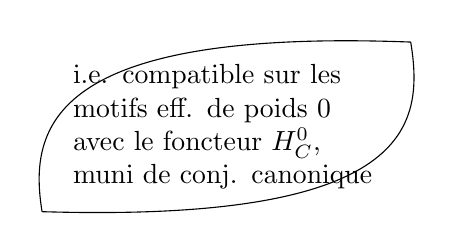
\begin{tikzpicture}
\node[align=left,text width=4cm,inner sep=8pt] (n) {i.e. compatible sur les motifs eff. de poids $0$ avec le foncteur $\unsure{H^0_{\mathbb C}}$, \unsure{muni de conj. canonique}};
\draw ([xshift=-3pt]n.south west) .. controls ([xshift=-8pt]n.west) and ([yshift=5pt]n.north west) .. (n.north east) .. controls ([xshift=5pt]n.east) and ([yshift=-4pt]n.south east) .. ([xshift=-3pt]n.south west);
\end{tikzpicture}}}
\unsure{C'est} tjs vrai si $M$ à degrés pairs, i.e. $j(\mu_2)=0$.

\uline{Proposition} 2. Conditions équivalentes

(i) $U$ est de la forme $U^{\unsure{\circ|0}}\times\mu_2$, $U^{\unsure{\circ|0}}$ un tore

(ii) $\varepsilon$ est \deleted{\unsure{un primitif}} un carré \inserted{dans $\operatorname{Hom}(G^{\unsure{\circ|0}},G_m)$}

(iii) $M_{\mathbb R}$ n'a pas de foncteur fibre \inserted{``non modifié''}, i.e. $\mathscr G_{\mathbb R}=\varnothing$.

Le fait que i) implique ii) \inserted{dans prop 1 ou prop. 2} résulte trivialt de \deleted{\unsure{l'implication de}} l'existence de $j$ avec $\varepsilon j(\lambda)=\lambda^2$, ainsi que le fait que $(1\,\mathrm{ii})\Longleftrightarrow(\text{non }\deleted{\unsure{1\,\mathrm{ii}}}\,2\,\mathrm{ii})$.

On a $(\mathrm{iii})\Rightarrow(\mathrm{ii})$, car plus précisément pour $\forall$ \deleted{\unsure{degré}} \inserted{objet} de \deleted{\unsure{degré}} \deleted{\unsure{tout}} \inserted{degré} \uline{impair} de $M_{\mathbb R}$, le \deleted{degré} \inserted{rg} doit être pair, comme il résulte de l'existence d'une forme alternée fondamentale. D'autre part i) $\Rightarrow$ (iii), car si $T$ est un tore compact sur $\mathbb R$, on a $H^{\unsure{2}}(\mathbb R,T)=0$ ! Enfin, si \deleted{\unsure{$G$}} \inserted{$M$} est à degrés pairs i.e. $j(\mu_2)=0$, donc $j=2j'$ et $\varepsilon j'=\mathrm{id}$, donc on a (ii).

\uline{Cor} Si $M$ est quelconque, la sous-catégorie \inserted{motivique} $M^{\text{pair}}$ \deleted{\unsure{satisf.}} \unsure{càd} qui correspond à $G/\deleted{\unsure{I}}j(\mu_2))$ \deleted{\unsure{est}} admet un $\mathbb R$-foncteur fibre.
\mspage{116}

\scanpage{118}
\deleted{Page 33. Ligne -9 à -1, remplacer le texte par le suivant:

« \uline{Remarques} 7.10. a) Lorsque $G$ est à fibres connexes, alors on peut dans c) abandonner l'hypothèse que les \deleted{$\unsure{p}$} $\inserted{{}_{\unsure{p^\nu|p^n}}}H'$ soient séparés. En effet, avec les réductions faites dans la démonstration, on peut supposer $u$ bijectif, donc $H$ à fibres connexes, donc $H$ séparé en vertu du théorème de séparation de Raynaud (Exp $\mathrm{VI}_{\mathrm B}$\quad).

b) D'autre part, des exemples de Raynaud montrent qu'on ne peut en général dans c) abandonner ni l'hypothèse que les $\inserted{{}_{\unsure{p^\nu|p^n}}}G'$ soient finis sur $S'$, ni que les $\inserted{{}_{\unsure{p^\nu|p^n}}}H'$ soient séparés sur $S'$.

c) \inserted{On peut montrer que} \unsure{La|la} conclusion de a) est encore valable si, au lieu de supposer $G$ à fibres connexes, on le suppose de type multiplicatif; \deleted{\unsure{alors}} tout monomorphisme $u:G\to H$ de $S$-préschémas en groupes\deleted{\unsure{à}} de présentation finie, avec $G$ de type multiplicatif, \deleted{\unsure{u}} est une immersion. »

Ligne 14, lire $S'$ au lieu de $S$.}

Page 35, ligne 9, 10, supprimer ``lisse sur $k$''.
\mspage{117}

\scanpage{119}
\uline{Cor} Dans le cas de la prop 2, \deleted{la catégorie} on a
\[
G^{\unsure{\circ|0}}\simeq U^{\unsure{\circ|0}}\times G_m,\quad\varepsilon=\operatorname{pr}_2,\quad j(\lambda)=\deleted{\unsure{\operatorname{pr}_2(\lambda)^2}}\operatorname{inj}_{\unsure{1|2}}(\lambda)^2.
\]
La structure \deleted{motivique 1) 2) 3)} de catégorie tannakienne de $M_{\mathbb R}$ est connue totalement par la connaissance de $G$ et l'élém de $H^2(\mathbb R,\unsure{U})$ caractéristique, qui \deleted{\unsure{provient}} \deleted{\unsure{est}} l'unique élém non nul de $H^2(\mathbb R,U)$, correspondant à l'unique élément non nul de $H^2(\mathbb R,\mu_2)$. Il existe un \deleted{élém} objet $E$ de $M_{\mathbb R}$ \deleted{\unsure{de}} de degré 1, rang 2, \deleted{\unsure{non trivial}} tel que la sous-catégorie tannakienne \deleted{$\unsure{M'}$} $M'$ qu'il engendre sera déjà $\mathbb R$-tordue, et \deleted{\unsure{correspond à un quotient}} \deleted{\unsure{qui}} \unsure{par} $U^{\unsure{\circ|0}}$ ``y opère \uline{trivialt}''.

Dans le cas favorable $\mathscr G_{\mathbb R}\ne\varnothing$, \margin{\inserted{i.e. $U$ un tore} \deleted{\unsure{à degrés pairs}}} l'ens \deleted{$\operatorname{Ob}\mathscr G_{\mathbb R}$} \inserted{$H^0(\mathscr G_{\mathbb R})$ des objets à isom près de $\mathscr G_{\mathbb R}$} est un \deleted{ens principal homogène} \inserted{torseur} sous le groupe $H^1(\mathbb R,U)$, qui lui-même est isom. can. à ${}_2U(\mathbb R)\underset{\text{non can.}}{\simeq}(\mathbb Z/2\mathbb Z)^{\dim U}$. D'autre part, à chaque élém de $\operatorname{Ob}\mathscr G_{\mathbb R}$ correspond une \deleted{structure de \unsure{fonctorialité}} \inserted{structure polarisante} sur $G^{\unsure{\circ|0}}$, définie par un hom
\diagram{\begin{tikzcd}
\mu_{2\mathbb C}\arrow[r,"i_1"] & G^{\unsure{\circ|0}}_{\mathbb C}
\end{tikzcd}}
tel que $\varepsilon_{\mathbb R}i_1=\mathrm{id}$, $i_1\bar i_1=j_{\mathbb R}$, et l'ens de ces structures est égalemt un torseur sous ${}_2U(\mathbb R)$. L'application
\diagram{\begin{tikzcd}
H^0(\mathscr G_{\mathbb R})\arrow[r] & \operatorname{Pol}(\mathscr G_{\mathbb R})
\end{tikzcd}}
est compatible avec l'opération de ${}_2U(\mathbb R)$, \uline{donc bijective}. Donc les $\mathbb R$-foncteurs fibres à isom
\mspage{118}

\scanpage{120}
\margin{78}
and since $\phi_k\ne0$ in $Q'$, $f_nQ'=Q$, then $\dfrac{\phi_0}{\phi_k},\ldots,\dfrac{\phi_T}{\phi_k}$, and with them $F_1$ and $F_2$ are regular in $Q'$; from the relations $F_2(Q')=F_2(Q)\ne0$ follows the regularity of $R$ in $Q'$.

Let us now show that, for large $n$, the mapping $f_n$ becomes one-to-one. The equation $\unsure{\varphi^{n\eta_e}|\omega^{n\eta_e}}=0$ will give a cross-section of the variety $V^{(n)}$ by some hyperplane, not containing $V^{(n)}$. Evidently, this cross-section is the image of $s$-$1$-dimensional subvariety $\mathcal E_\varphi$ of the variety $V$ (the equation $\mathcal E_\varphi$ in $U^{(i)}$ - the set $\phi^{(i)}=0$).

According to the induction hypothesis, there exists $m(\mathcal E_\varphi)$ such that the elements of the group \margin{\unsure{if}} $H^0(\mathcal E_\varphi,O_{\mathcal E_\varphi}[mE']_{\mathcal E_\varphi})$ will give a biregular imbedding of the variety $\mathcal E_\varphi$ in a projective space. From the exact sequence (19) we obtain that this imbedding of the variety $\mathcal E_\varphi$ is the restriction of the mapping $f_m:V\to V^{(m)}$ on the subvariety $\mathcal E_\varphi$. We obtain, in particular that the image $\mathcal E_\varphi$ by the mapping $f_m$ possesses a dimension $s$-$1$. Hence it follows that the cross-section of the variety $V^{(m)}$ by a hyperplane, not containing $V^{(m)}$, possesses a dimension $s$-$1$ and, consequently,
\[
\dim V^{(m)}=s.
\]
\mspage{119}

\scanpage{121}
près et les structures de polarisation sur $G^{\unsure{\circ|0}}$ se \uline{déterminent mutuellement}.

\deleted{\unsure{Donc}} [À voir: l'ens des autom de $(G^{\unsure{\circ|0}}_{\mathbb R},\varepsilon_{\mathbb R},j_{\mathbb R})$ voire $(G^{\unsure{\circ|0}}_{\unsure{Q}},\varepsilon,\unsure{j|\mu})$, voire $(G,\varepsilon,\unsure{j|\mu})$ opère-t-il transitivement sur $\operatorname{Pol}(G)$ ? \deleted{Par exemple} est-il possible \deleted{\unsure{ici}} de distinguer \deleted{\unsure{au moyen de}} \inserted{une} \deleted{\unsure{toujours, y a-t-il}} polarisation ou un paquet de polarisations préférentielles ?]

Prenons p.ex. une catégorie de Motifs géométriques sur $\mathbb F_q$, $q=p^n$, \deleted{\unsure{et}} Alors \deleted{\unsure{donc}} il y a une classe de conjugaison d'homs
\diagram{\begin{tikzcd}
\unsure{i}:G_{m\mathbb C}\arrow[r] & G_{\mathbb C}
\end{tikzcd}}
distinguée, avec
\[
\bar i i=j,\qquad\varepsilon i=\mathrm{id}
\]
\margin{N.B. $i$ et \unsure{les conjugués} \inserted{\unsure{distincts}} sur $Q$, (\unsure{au nb} \deleted{\unsure{de}} $\unsure{2n}$, si $[K:Q]=n$ \unsure{engendrent} $\operatorname{Hom}(G_{m\mathbb C},G^{\unsure{\circ|0}}_{\mathbb C})$}
définie, \deleted{par} si $G$ commutatif: $M\subset L$ \margin{$L$ quadratique tot. imag., $K$ tot. réelle,} par la
\figure{\begin{tikzpicture}[every node/.style={align=left}]
\node[draw,ellipse,inner sep=5pt] (f) at (5,1.7) {forme};
\node[draw,rounded corners=12pt,text width=4cm,inner sep=5pt] (a) at (0,0) {\deleted{\unsure{est}}\par \uuline{\unsure{caveat}} $\longrightarrow$ cette forme \deleted{\unsure{en général}} n'est pas tjrs ! à valeurs entières \unsure{même si}};
\node[draw,rounded corners=15pt,text width=4cm,inner sep=5pt] (b) at (0,-3.7) {$\unsure{M}$ si $j=0$, ex: prendre $q=p\ne2$\par $L=Q(\unsure{\sqrt{-p}|\sqrt p})$, tel que nb de classes de $L$ soit $1$, p.ex.\par $p:3,7,11,\ldots$};
\draw (a.north east)--(f.west);
\draw (a.south)--(b.north);
\end{tikzpicture}}
\[
\lambda\longmapsto\frac1n v_{\mathfrak p}(\lambda),
\]
si $\mathfrak p$ est un idéal premier de $L$ sur $p$.
\[
[\ v_p(\lambda)v_p(\bar\lambda)=v_p(\lambda\bar\lambda)=v_p(q^{j^*(\lambda)})=j^*(\lambda);\quad v_p(q)=1\ ].
\]
En fait, il convient de ``normaliser'' $G_{\mathbb C}$ \inserted{\fbox{sur $Q$ !}} \unsure{choix} d'un tore; (NB. Un autom de $G^{\unsure{\circ|0}}$ qui \deleted{induit} respecte $i$ est l'identité !). La structure d'effectivité sur $M$ est déterminée grâce à $i$, celle des $M_k$ ($k$ ext. de $Q$) en particulier de $M_{\mathbb R}$, $M_{\mathbb C}$, par la considération des systèmes de leurs conjugués
\mspage{120}

\scanpage{122}
\margin{77}
or, what comes to the same thing, the values
\[
\frac{\unsure{\Phi|\phi}_0}{\unsure{\Phi|\phi}_k}(Q),\ldots,\frac{\unsure{\Phi|\phi}_T}{\unsure{\Phi|\phi}_k}(Q)
\]
from which it follows that
\[
(\unsure{\Phi|\phi}_0^{(i)}(Q'),\ldots,\unsure{\Phi|\phi}_T^{(i)}(Q'))=(x_0(Q),\ldots,x_T(Q))
\]
\margin{p. 210} and
\[
Q=f_nQ'
\]

It is easy to show that $f_n$ is a continuous mapping (in Zariski's topology) and even a regular one. The latter follows from the fact that, in $Q\in V^{(n)}$ ($x_k\ne0$ at $Q$), any regular function $R$ has the form
\[
R=\frac{F_1\left(\dfrac{x_0}{x_k},\ldots,\dfrac{x_T}{x_k}\right)}{F_2\left(\dfrac{x_0}{x_k},\ldots,\dfrac{x_T}{x_k}\right)}
\]
where $F_1$ and $F_2$ are polynomials and $F_2(Q)\ne0$; the corresponding function on $V$ will be
\margin{\unsure{1)}}
\[
R'=\frac{F_1\left(\dfrac{\unsure{\Phi|\phi}_0}{\unsure{\Phi|\phi}_k},\ldots,\dfrac{\unsure{\Phi|\phi}_T}{\unsure{\Phi|\phi}_k}\right)}{F_2\left(\dfrac{\unsure{\Phi|\phi}_0}{\unsure{\Phi|\phi}_k},\ldots,\dfrac{\unsure{\Phi|\phi}_T}{\unsure{\Phi|\phi}_k}\right)}
\]
\mspage{121}

\scanpage{123}
de $i$. \deleted{\unsure{Question la structure de polarité est elle associée à} $i|\mu_2$ ?}
Donc, grâce à cette circonstance spéciale, il y a des classes de \deleted{polarité} structures polarisantes privilégiées dans $G$: les $i|\mu_2$ avec $i$ dans la classe ci-dessus.
\margin{\diagram{\begin{tikzcd}
G_{m\mathbb C}\arrow[r,dash,"i"] & G_{\mathbb C}
\end{tikzcd}}}

Quel est l'arbitraire ? On constate que l'ens \inserted{des} $(i-i'$ \deleted{\unsure{correspond à} $v_{\mathfrak p'}(\lambda)-v_{\mathfrak p}(\lambda)$} définit un sous-groupe \uline{d'indice fini} de $\operatorname{Hom}(G_{m\mathbb C},G^{\unsure{\circ|0}}_{\mathbb C})$, mais cela ne donne aucune indication sur le comportement des $i_0-i_0'$, où l'indice $0$ désigne la \unsure{contr.|restr.} à $\mu_2$. Question semble secondaire.
\margin{\diagram{\begin{tikzcd}
G_{m\mathbb C}\arrow[r,"i'"] & G_{\mathbb C}
\end{tikzcd}}}

\margin{\figure{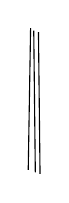
\begin{tikzpicture}
\draw (0,0)--(0.03,1.8);\draw (0.09,-0.03)--(0.07,1.77);\draw (0.15,-0.05)--(0.13,1.75);
\end{tikzpicture}}}
En tous cas, on a \deleted{des} \inserted{un} paquet de $\mathbb R$-foncteurs fibres privilégiés, définis en termes des différents $i$.

\figure{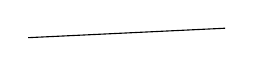
\begin{tikzpicture}\draw (0,0)--(2.5,0.12);\end{tikzpicture}}

Autre structure spécifique sur le $G$ provenant d'un corps fini: d'après la façon de l'écrire $G_{\mathbb C}:D_{\mathbb C}(M)$, $M\subset L^*$, comme $L$ est stable par conjugaison complexe, qui commute à $\operatorname{Gal}(L/Q)$, \unsure{on trouve} dans $M$ donc $G$ une involution canonique, notée
\[
u\longmapsto u'
\]
Dans $\operatorname{Ker}j^*$ c'est la symétrie, d'autre part sur $\operatorname{Im}j$ c'est l'identité, ce qui suffit pratiquement à la déterminer. Sur $\operatorname{Hom}(G_{m\mathbb C},G_{\mathbb C})$ $u\mapsto u'$ induit la conjugaison complexe.
\mspage{122}

\scanpage{124}
\margin{76}
of the field $k(\dfrac{x_0}{x_k},\ldots,\dfrac{x_T}{x_k})$ in $(k,\infty)$ and even the homomorphism of the field $k(\dfrac{\phi_0}{\phi_k},\ldots,\dfrac{\phi_T}{\phi_k})$ in $(k,\infty)$. The last homomorphism can be extended to the point of the field $k(V)$, and, in view of the completeness of $V$, this point possesses some center $Q'$ on $V$. Let $k_1$ be such that $\phi_{k_1}\ne0$ in $Q'$. Then $F=\dfrac{\phi_k}{\phi_{k_1}}$ is a regular function in $Q'$ (since, if $Q'\in U^{(i)}$, then $F=\dfrac{\phi_k^{(i)}}{\phi_{k_1}^{(i)}}$ and $\phi_k^{(i)}$, $\phi_{k_1}^{(i)}\in O_{V,Q'}$, $\phi_{k_1}^{(i)}(Q')\ne0$). If $\phi_k=0$ in $Q'$, then $F(Q')=0$ and
\[
\frac{1}{F(Q')}=\frac{\unsure{\Phi|\phi}_{k_1}}{\unsure{\Phi|\phi}_k}(Q')=\infty
\]
But
\[
\frac{\unsure{\Phi|\phi}_{k_1}}{\unsure{\Phi|\phi}_k}(Q')=\frac{\unsure{\Phi|\phi}_{k_1}}{\unsure{\Phi|\phi}_k}(Q)=\frac{x_{k_1}}{x_k}(Q)\ne\infty
\]
Therefore, $\phi_k\ne0$ in $Q'$. But then the functions
\[
\frac{\unsure{\Phi|\phi}_0}{\unsure{\Phi|\phi}_k},\ldots,\frac{\unsure{\Phi|\phi}_T}{\unsure{\Phi|\phi}_k}
\]
are regular in $Q'$ and take there the values
\[
\frac{x_0}{x_k}(Q),\ldots,\frac{x_T}{x_k}(Q)
\]
\mspage{123}

\scanpage{125}
Il \unsure{ne|me} semble pas que cette involution \unsure{corresponde} à une involution dans la \uline{gerbe} $\mathscr G$ associée à $M$ (\unsure{on} \deleted{\unsure{semble}} \deleted{\unsure{pas}} n'a pas la propriété de \unsure{covariance|conservation} voulue \unsure{p.r.|par.} à l'élément fondamental \unsure{conjectural} dans $H^2(Q,\deleted{\unsure{G}}U)$ $\unsure{h|b}$, qui serait \deleted{d'ordre $2$} d'ordre \unsure{divisant} $2$\ldots).
\mspage{124}

\scanpage{126}
\margin{74}
\[
H^1(\mathcal E_\varphi,O_{\mathcal E_\varphi}[nE]_{\mathcal E_\varphi})=0
\]
we obtain an exact sequence
\diagram{\begin{tikzcd}
H^0(V,O_V[nE]) \arrow[r,"r^*"] & H^0(\mathcal E_\varphi,O_{\mathcal E_\varphi}[nE]_{\mathcal E_\varphi}) \arrow[r] & 0
\end{tikzcd}}\hfill(19)

Let us assume that there would exist a point $P\in\mathcal E_\varphi$ such that in $P$ any cross-section $\phi\in H^0(V,O_V[nE])$ satisfies the condition: if $P\in U^{(i)}$, then $\phi^{(i)}(P)=0$. Since any cross-section $\phi'\in H^0(\mathcal E_\varphi,O_{\mathcal E_\varphi}[nE]_{\mathcal E_\varphi})$ can be presented in the form $\phi'=r^*\phi$ or $\phi'^{(i)}=r\phi^{(i)}$ and $r$ in the stalk over $P$ is a homomorphism of restriction of functions; then $\phi'^{(i)}(P)=0$. But this contradicts the fact that, at $n\ge n(\mathcal E_\varphi)$, the elements of the group $H^0(\mathcal E_\varphi,O_{\mathcal E_\varphi}[nE]_{\mathcal E_\varphi})$ generate the stalk of the sheaf $O_{\mathcal E_\varphi}[nE]_{\mathcal E_\varphi}$ over any point $P\in\mathcal E_\varphi$. The lemma is proved.\ \rule{0.5em}{1em}

Let us come back to the proof of theorem 2. Put $E'=n_{\mathcal E}E$, where $n_{\mathcal E}$ is the number to which lemma 3 refers. Let $\phi_0,\ldots,\phi_T$ be the basis (not necessarily of linearly independent vectors) of the group $H^0(V,O_V[nE'])$.

Consider a mapping $f_n:\ V\to P^T$ ($P^T$ is a T-dimensional projective space), operating according to the rule: if $P\in V$, $P\in U^{(i)}$, then
\mspage{125}

\scanpage{128}
\uline{Définition} Soit $K/Q$ une extension \deleted{\unsure{algébrique}} \inserted{algébrique}. On dit que $K$ est tot. réel si pour tout $Q$-hom $\sigma:K\to C$, on a $\sigma(K)\subset\unsure{\mathbb R|R}$. On dit qu'un élément $\unsure{x|a}$ de $K$ est tot. réel \inserted{(resp. tot. $>0$, tot. $\ge0$)} si pour les $\sigma$ comme dessus, on a $\sigma(x)\in\unsure{\mathbb R|R}$ (resp. $\sigma(x)>0$, resp. $\sigma(x)\ge0$). Tot. (ou purement) imaginaire: \ldots.

\uline{Sorite} Pour que $x$ soit tot. réel, il \unsure{f. et s.} que $Q(x)\subset K$ le soit. Pour qu'il soit tot. $\ge0$, il faut et il suffit qu'il soit nul ou tot $>0$. Les éléments tot $\ge0$ \deleted{\unsure{forment}} \inserted{sont} les éléments $\ge0$ pour une relation d'ordre sur $K$. [On parlera de $x$ tot. $\ge y$ ou $x$ tot. $\le y$]. Si $K$ est engendré par des ss-corps $K_\alpha$, alors $K$ est tot. réel ssi les $K_\alpha$ le sont. Si \inserted{$K$ est engendré par des $x_\alpha$,} $K$ tot. réel ssi \deleted{\unsure{les élts}} les $x_\alpha$ le sont.

Il existe, pour $K$ donné, un plus grand ss-corps totalement réel de $K$, appelé la \uline{clôture tot. réelle} de $Q$ dans $K$. Soit $\deleted{K=}\overline Q\subset C$, et $\pi=\operatorname{Gal}(\unsure{\overline Q}/Q)$, enfin $\tau\in\pi$ la conjugaison complexe
\[
\tau\lambda=\overline\lambda\qquad\text{pour }\lambda\in\overline Q
\]
de sorte qu'on a
\[
\tau^2=1.
\]
Alors le ss-groupe $\pi'$ de $\pi$ qui \deleted{\unsure{invariante}} \inserted{correspond} à la clôture tot. réelle $\deleted{\unsure{de}}\mathbb K\deleted{\unsure{Q}}$ de $Q$ dans $\overline Q$ est \deleted{\unsure{le}} le ss-groupe \uline{invariant} \uline{fermé} engendré par $\tau$, i.e. le ss groupe invariant engendré par les ${}^{\sigma}\tau=\sigma\tau\sigma^{-1}$ $(\sigma\in\pi)$.
\margin{\diagram{\begin{tikzcd}[row sep=small]
A \arrow[d,dash] \\
\mathbb L \arrow[d,dash] \\
\mathbb K \arrow[d,dash] \\
Q
\end{tikzcd}}}
Considérons la plus grande extension abélienne $A$ de $\mathbb K$, dont le groupe de Galois est donc $H=\pi'/(\pi',\pi')$. \deleted{\unsure{En}} Sur
\mspage{127}

\scanpage{129}
\unsure{ce} groupe $G=\pi/\pi'=\operatorname{Gal}(\mathbb K/Q)$ opère continûment, et il est engendré topologiquement par les ${}^{\sigma}\overline\tau$ où $\overline\tau\in H$ est l'image de $\tau$, et $\sigma\in G$. Donc il \uline{est annulé par $2$}.

\margin{\figure{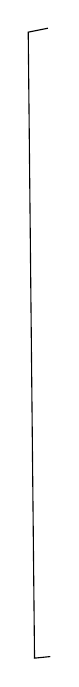
\begin{tikzpicture}\draw (0.25,8)--(0,7.95)--(0.08,0)--(0.28,0.02);\end{tikzpicture}}}
Soit $L$ une extension abélienne de $\mathbb K$, \deleted{\unsure{son groupe de Gal. $\Gamma$}} son groupe de Galois est donc un quotient $\Gamma$ de $H$; \deleted{Conditions} Supposons $L\ne \mathbb K$, i.e. $\Gamma\ne\{e\}$. Conditions équivalentes

(i) les $\sigma\tau\sigma^{-1}$ $(\sigma\in\pi)$ coïncident toutes sur $L$ (donc y coïncident avec $\tau:\lambda\to\overline\lambda$)

(ii) $L$ est une extension \uline{quadratique} de $\mathbb K$ \uline{galoisienne sur} $Q$.

\deleted{\illegible{5}}
\inserted{(iii) $L$ est une extension \uline{quadratique} \uline{purement imaginaire} de $\mathbb K$.}

De plus, une telle $L$ \deleted{existe et} est unique, [et d'ailleurs existe: il suffit de prendre une extension quadratique imaginaire $E$ de $Q$, \inserted{(p. ex. $Q(\sqrt{-1})$)} et $L=Q(\mathbb K,E)$ (p. ex. $L=\mathbb K(\sqrt{-1}))$].

\uline{Dém} (i)$\Rightarrow$(ii) Comme $\Gamma$ est engendré par les images \deleted{\unsure{des}} des ${}^{\sigma}\overline\tau$, \deleted{\unsure{il s}} et que l'hyp. de (i) signifie que ces images sont égales, on voit que (i) implique que $\Gamma$ est engendré par l'élémt $\overline\tau$ de \unsure{expos.} $|2$, donc est $\simeq Z/2Z$ (car $\Gamma\ne(e)$ par hypothèse). D'ailleurs, si un tel $\Gamma$ existe, \deleted{\unsure{il}} \inserted{il est} nécessairement égal à $H_G$ car \deleted{\unsure{lui}} c'est un quotient de $H_G$, et l'argument précédent montre que \deleted{\unsure{ce}} $H_G$ est engendré par un élément d'ordre $|2$. \deleted{\unsure{On}} \deleted{il existe bel et} Il en résulte aussitôt que $L$ est galoisien sur $Q$, donc (i)$\Rightarrow$(ii). D'autre part, (ii)$\Rightarrow$(i), car (ii) implique que $\Gamma\simeq Z/2Z$ \inserted{et que $G$ y opère}, et comme $\Gamma$ est engendré par les images des $\sigma\tau\sigma^{-1}={}^{\sigma}\tau$, i.e. par les ${}^{\sigma}\overline\tau$, on voit que $\overline\tau$ (donc les ${}^{\sigma}\overline\tau$) sont tous égaux à l'unique élément non nul de $\Gamma$.

((i), (ii))$\Longleftrightarrow$(iii) Car du moment que $L$ est quadratique sur $\mathbb K$, la condition (i) sur les $\sigma\tau\sigma^{-1}$ est évidemment équivalente à (iii)
\mspage{128}

\scanpage{130}
\uline{Corollaire} Soit $L$ un ss-corps de $\overline Q$. Pour qu'on ait $L\subset\mathbb L$, il f. et s. que $L$ soit tot réel, ou extension quadratique purement imaginaire d'un corps tot. réel.

Suffisance triviale par (iii). Nécessité: Par théorème de Galois, $L$ est une extension de degré $1$ ou $2$ du corps tot. réel $K=L\cap\mathbb K$, et il reste à prouver que lorsque $L$ en est une extension quadratique, cette dernière est \unsure{tot\textsuperscript{t}|tot.} \uline{imaginaire}.
\margin{\diagram{\begin{tikzcd}[row sep=small,column sep=small]
\mathbb K \arrow[r,dash] \arrow[d,dash] & \mathbb K(L) \arrow[r,dash] \arrow[d,dash] & \mathbb L \\
K=\mathbb K\cap\unsure{L|\mathbb L} \arrow[r,dash] \arrow[d,dash] & L \\
Q
\end{tikzcd}}}
\deleted{\unsure{On a}} Or \deleted{\unsure{on voit aisément que}} on est ramené à prouver
\deleted{\uline{Lemme} Soit $L$ une extension quadratique d'un corps tot. réel $K$ de $\unsure{L|\mathbb L}$}
(quitte à remplacer $L$ par un conjugué, \inserted{ce qui ne dérange pas $\unsure{K|\mathbb K}$,}) que $L$ est imaginaire. Or s'il était réel, comme $\mathbb K$ l'est, $\mathbb K(L)$ le serait, or $\mathbb K(L)=\mathbb L$, absurde.

\uline{NB} $\mathbb L$ est la plus grande extension galoisienne de $Q$, telle que dans son groupe de Galois $G'$, l'image de $\tau$ (conjugaison complexe) soit \uline{centrale}. Donc $\mathbb L$ contient l'extension abélienne maximale de $Q$, i.e. le corps des racines de l'unité.
\mspage{129}

\scanpage{131}
\uline{Proposition} Soit $Q\in Q^*$, et soit $\lambda\in C$ un nombre algébrique. Conditions équivalentes

(a) Pour tout conjugué $\lambda_\alpha$ de $\lambda$, on a $\lambda_\alpha\overline\lambda_\alpha=Q$ i.e. $|\lambda_\alpha|^2=\unsure{Q}$.

(b) \deleted{\unsure{Réciproquement}} Il existe un corps \inserted{de nbs} \uline{totalement réel} $K$, tel que \deleted{\unsure{on a}} $K(\lambda)$ soit égal à $K$ ou une extension \uline{quadratique} purement imaginaire de $K$, et on a $\lambda\overline\lambda=Q$ i.e. $|\lambda|^2=Q$.

(b') Comme (b), avec $K=Q(a)\deleted{\unsure{=Q(\lambda)}}$, où $a=\lambda+\overline\lambda=\lambda+\dfrac Q\lambda$.

(b'') Il existe un nombre algébrique \deleted{\unsure{a}} \uline{tot} \uline{réel} $a$, avec \deleted{\unsure{$a^2-4Q$ nul}} $4Q-a^2$ nul ou totalement positif, tel que $\lambda$ satisfasse une équation
\[
\lambda^2-a\lambda+Q=0
\]

(c) Soit $\mathbb K$ l'extension alg. tot. réelle maximale de $Q$, et $\mathbb L$ l'unique extension quadratique de $\mathbb K$, galoisienne sur $Q$. On a $\lambda\in\mathbb L$, et $\deleted{\unsure{K\lambda}}\lambda\overline\lambda=Q$ i.e. $|\lambda|^2=Q$.

\uline{Dém}

a)$\Longrightarrow$b'') Posons $a=\lambda+\overline\lambda=\lambda+\dfrac Q\lambda$. Je dis que $a$ \uline{est tot. réel}. En effet, les conjugués de $a$ sont les $\deleted{\unsure{\sigma}}a_\alpha=\deleted{\unsure{\sigma}}\lambda_\alpha+\dfrac Q{\deleted{\unsure{\sigma}}\lambda_\alpha}$, or par hypothèse $\lambda_\alpha\overline\lambda_\alpha=Q$ donc $a_\alpha=\lambda_\alpha+\overline\lambda_\alpha\in\unsure{\mathbb R|R}$. D'autre part, $\lambda$ est solution de l'équation
\inserted{$(T-\lambda)(T-\overline\lambda)=0$ i.e.}
\[
\unsure{T^2|T}-aT+Q=0,
\]
et par suite $\lambda_\alpha$ est solution de l'équation $T^2-a_\alpha T+Q_{\unsure{\alpha}}=0$, \deleted{de plus} l'autre solution étant $\dfrac Q{\lambda_\alpha}$ \inserted{(qui peut être égale à $\lambda_\alpha$)}, \deleted{\unsure{donc}} comme $\lambda_\alpha\overline\lambda_\alpha=Q$, les deux solutions sont $\lambda_\alpha$ et $\overline\lambda_\alpha$, donc complexes conjuguées. Cela montre que $a_\alpha^2-4Q\le0$, \deleted{\unsure{donc}} \inserted{i.e.} $4Q-a_\alpha^2\ge0$, donc $4Q-a^2$ est tot positif.

b'')$\Longrightarrow$b') Il est évident que $\lambda$ est de degré au plus deux sur \inserted{le corps tot. réel} $Q(a)$, \deleted{\unsure{de plus comme}} \deleted{$\unsure{\lambda\in Q(a)}$} \inserted{et $Q(\lambda)\supset Q(a)$ [car $a=\lambda+\dfrac Q\lambda$].} \deleted{\unsure{car que}} Comme $a^2-4Q\le0$, les solutions de l'équation $T^2-aT+Q=0$ sont $\lambda$ et $\overline\lambda$ \inserted{(cf lemme plus bas)}, et on a $\lambda\overline\lambda=Q$, $\lambda+\overline\lambda=a$.
\mspage{130}

\scanpage{132}
\inserted{\unsure{Enfin|\deleted{Enfin}}} Il faut prouver que si $\lambda\notin K$ i.e. $a^2-4Q\ne0$ (cf lemme plus bas), alors \deleted{\unsure{$\lambda$ est purement}} $Q(\lambda)$ est purement imaginaire, i.e. les $\lambda_\alpha$ sont tous non réels. \deleted{Cela signifie que les} \inserted{Comme $\lambda_\alpha$ est solution} de l'équation $\unsure{T^2|T}-a_\alpha T+Q=0$, cela signifie que $a_\alpha^2-4Q<0$, ce qui résulte du fait que $4Q-a^2$ est tot $\ge0$.

b')$\Rightarrow$b) trivial, \deleted{\unsure{puisque}}

b)$\Rightarrow$c) trivial, car $\mathbb K(\lambda)$ est égal à $\mathbb K$ ou est une ext. quadratique purement imaginaire de $\unsure{\mathbb K|K}$.

c)$\Longrightarrow$a) car si $\lambda_\alpha=\sigma_\alpha(\lambda)$, on aura \deleted{\unsure{que $\overline\lambda_\alpha$ est}} \inserted{$\lambda_\alpha\in\mathbb L$, donc,} $\overline\lambda_\alpha$ est l'unique \deleted{\unsure{$\lambda$}} conjugué de $\lambda_\alpha$ sur $\unsure{\mathbb K|K}$, \deleted{\unsure{et}} donc
\[
\lambda_\alpha\overline\lambda_\alpha=N_{\mathbb L/\mathbb K}(\lambda_\alpha)=N_{\mathbb L/\mathbb K}(\lambda)=\lambda\overline\lambda=Q.
\]

\deleted{\uline{Corollaire} Soit $L\subset\mathbb L$, \inserted{Supposons $Q\in Q^{*+}$, $L$ fini sur $Q$, $L$ non \deleted{\unsure{totalement}} réel (i.e. non tot. réel)} Alors $L$ est engendré par un $\lambda$ tel que $\lambda\overline\lambda=Q$. Si $Q\in Z$, on peut supposer \deleted{\unsure{encore}} que $\lambda$ est entier.}

\uline{Remarque} Soit $K$ une extension finie tot. réelle de $Q$, et $Q\in Q^{\unsure{*+}}$, $Q>1$. Je dis qu'il existe alors une extension quadr. purement imaginaire $L$ de $K$, \deleted{telle que} et un entier $i\ge0$, \deleted{tels que} tels que $\unsure{L|K}$ soit engendré \inserted{sur $Q$} par un élément $\lambda$ tel que $\lambda\overline\lambda=Q^i$ i.e. $|\lambda|^2=Q^i$. Si $Q\in Z$, on peut $\overline{\mathrm m}$ prendre $\lambda$ entier algébrique.

Dém. Soit $a\in K$ tel que $\unsure{K}=Q(a)$. \inserted{on peut supposer $a$ entier.} Soit $i$ assez grand pour que $\deleted{\unsure{Q^i}}4Q^i-a^2$ soit tot. $>0$ (\deleted{\unsure{cela est possible}} certes, car $Q\in Q$, $Q>1$). Soit $\lambda$ solution de l'équation $\lambda^2-a\lambda+Q^i=0$. Il satisfait à la condition voulue; si $Q$ est entier, il est entier, à l'évident.
\mspage{131}

\scanpage{133}
Notons que $\lambda'=\lambda^{1/i}$ \unsure{sera} aussi dans $\mathbb L$ (car $\lambda\overline\lambda=Q\deleted{\unsure{i}}$, et de $\unsure{\overline{\mathrm m}|=}$ pour ses conjugués\ldots), donc on voit aussi qu'il existe un $\lambda'$ \deleted{\unsure{tel que}} $\in\mathbb L$, avec $\deleted{\unsure{f}}\lambda'\overline{\lambda'}=|\lambda'|^2=Q$, tel que $Q(\lambda')$ soit \deleted{\unsure{p}} \inserted{(purement)} imaginaire et \uline{contenant} $K$; de plus, si $Q$ est entier, on peut prendre $\lambda'$ entier.
\mspage{132}

\scanpage{135}
\uline{Groupes de Galois motiviques commutatifs.}
\margin{D R}

$k$ corps

$M$ catégorie des (iso)-motifs ($\frac12$ simples) sur $k$

$G$ lien de $M$, \deleted{\unsure{supposé commutatif}}

$\mathscr G$ gerbe des \deleted{\unsure{les}} foncteurs fibres de $M$

$\deleted{\unsure{\mathscr G}}$
\margin{D R}
$\deleted{\unsure{\mathscr G\to}}\quad\uline{M_0\subset M}$, catégorie \deleted{\unsure{des objets}} \inserted{engendrée} par $Q(1)$ de Tate

$\mathscr G_0$, $G_0=G_m$ gerbe et lien correspondants

\diagram{\begin{tikzcd}
\mathscr G \arrow[r] & \mathscr G_0 \\
G \arrow[r,"\varepsilon","\uline{\text{épimorphisme}}"'] & G_m
\end{tikzcd}}
$\mathscr G_0$ est trivialisée i.e. on se donne une section, correspondant à un foncteur-fibre $\varphi$ \deleted{$Q(1)\longrightarrow Q$} choisi sur $M_0$

[\uline{NB} Comme $H^1(Q,G_m)=0$, deux foncteurs fibres sur $M_0$ sont \inserted{\deleted{\unsure{can.}}} isomorphes]
\margin{D R}

Une trivialisation de $\mathscr G_0$ permet de \uline{\unsure{rétrécir|restreindre}} le lien de $\mathscr G$ de $G$ à $\operatorname{Ker}\varepsilon=\unsure{U}$: on prend les foncteurs fibres \uline{munis} d'un isom. de leur restriction à $M_0$ avec le foncteur fibre fixé sur $M_0$. On trouve une nouvelle gerbe $\mathscr G_\varphi$ de lien $U$.
\margin{\uline{\unsure{cf|voir} Giraud?}}
\margin{D R}

Soit $M'$ la ss-catégorie de $M$ formée des objets $M$ tels que les $\otimes^{\unsure{n|\bullet}}(M+\check M)$ soient combinaisons d'un nb fini d'objets simples; \inserted{$\mathscr G'$ la gerbe associée, $G'$ le lien.} On en déduit
\margin{D R}
\diagram{\begin{tikzcd}
& & \mathscr G \arrow[r] & \mathscr G' \arrow[r,dash] & 1 \\
1 \arrow[r,dash] & G^{\unsure{\circ|0}} \arrow[r,dash] & G \arrow[r,"\text{épim}"'] & G' \arrow[r,dash] & 1
\end{tikzcd}}
\margin{D R}
\margin{\figure{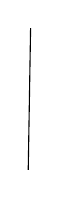
\begin{tikzpicture}\draw (0,0)--(0.03,1.8);\end{tikzpicture}}}
le noyau de $G\to G'$ est la ``composante neutre'' $G^{\unsure{\circ|0}}$.
\margin{D R}

D'autre part, l'on sait que $M'$ est équivalente à une ss-catégorie \inserted{pleinement fidèle} des $Q$-\unsure{vectoriels} étales sur $k$. La donnée d'une clôture algébrique $\overline k$ de $k$ fournit un
\margin{D R}
\mspage{134}

\scanpage{137}
foncteur fibre \inserted{$\psi=\psi_{\overline k}$} sur $M'$, i.e. une section de $\mathscr G'$, d'où une \deleted{\unsure{restriction}} \deleted{\unsure{restreinte}} gerbe $\mathscr G_\psi$ de lien $G^{\unsure{\circ|0}}$, qui \deleted{\unsure{donc}} est \deleted{liée} reliée à la gerbe $\mathscr G$ de lien $G$ via $G^{\unsure{\circ|0}}\hookrightarrow G$.

\uline{NB} En général, $H^1(Q,\Gamma)\ne1$, donc il y a ici un choix \uline{très} \uuline{particulier} de trivialisation de \uline{la gerbe $\unsure{M'|M''}$}.

Considérons enfin la \deleted{gerbe} \inserted{ss-catégorie tensorielle de $M$} \inserted{$M^{(0)}$} engendrée par $M_0$ et $M'$: c'est la catégorie formée des sommes directes
\[
\sum_{i\in Z}V_i(i),
\]
où les $V_i$ sont $\in M'$, et les $V_i\in M'$ sont tous nuls sauf un nb fini
\margin{\figure{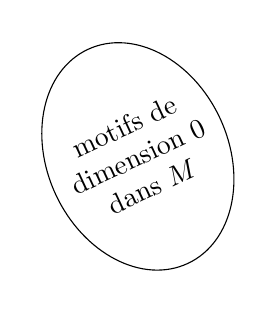
\begin{tikzpicture}\draw[rotate=25] (0,0) ellipse (1.15 and 1.5);\node[rotate=25,align=center] at (0,0) {\uline{\unsure{motifs de}}\\\uline{\unsure{dimension} $0$}\\\uline{dans $M$}};\end{tikzpicture}}}
[NB
\[
\left(\sum V_i(i)\right)\otimes\left(\sum W_j(j)\right)=\sum_n\left(\sum_{i+j=n}V_i\otimes W_j\right)(n),\qquad
\left(\sum V_i(i)\right)^\vee=\sum\check V_{\unsure{i|-i}}(-i)
\]
]
On trouve un foncteur fibre
\diagram{\begin{tikzcd}
\displaystyle\sum_{i\in Z}V_i(\unsure{k|i}) \arrow[r] & \displaystyle\sum V_i(\overline k)
\end{tikzcd}},
\margin{\diagram{\begin{tikzcd}[row sep=small,column sep=small]
M_0 & M^{(0)} \arrow[l,dash] \\
& M' \arrow[u,hook]
\end{tikzcd}}}
$\deleted{\unsure{a}}\mathscr G^{(0)}$, $\underset{\text{groupe}}{G^{(0)}}\simeq G'\times G_m$

\diagram{\begin{tikzcd}
& & \mathscr G \arrow[r] & \mathscr G^{(0)} \\
1 \arrow[r] & U \arrow[r,phantom,"\unsure{\text{—}|\longrightarrow}"] & G \arrow[r,phantom,"\unsure{\text{—}|\longrightarrow}"] & G^{(0)}=G_m\times G' \arrow[r,dash] & 1
\end{tikzcd}}
On trouve une \deleted{\unsure{restriction}} \inserted{gerbe} $\mathscr G_\chi$ sous $U$, reliée à la gerbe $\mathscr G$ sur $G$ \deleted{\unsure{par}} \unsure{et|via} $U\hookrightarrow G$.
\mspage{136}

\scanpage{138}
\mspage{137}
\margin{- 16 -}
\margin{n° 505}
\uline{P. 129}, ligne 3 du haut, remplacer ``métrisable'' par ``séparé''. Ligne 19 du bas, remplacer ``\uline{métrisable}'' par ``\uline{séparé}''.

Lignes 2 à 10 du bas, remplacer par:

Considérons en effet l'application surjective $f:\{0,1\}^{\uuline{N}}\to I$ qui, à tout point $(\unsure{\epsilon|e}_n)_{n\ge0}$ avec $\unsure{\epsilon|e}_n=0$ ou $\unsure{\epsilon|e}_n=1$, fait correspondre le nombre $\sum_{n=0}^{\infty}\unsure{\epsilon|e}_n2^{-n}$ ayant $(\unsure{\epsilon|e}_n)$ pour développement dyadique. Soit $D$ l'ensemble dénombrable dans $\{0,1\}^{\uuline{N}}$ formé des suites autres que la suite $0$, n'ayant qu'un nombre fini de termes $\ne0$; $P=\{0,1\}^{\uuline{N}}-D$ est un espace polonais éparpillé (n° 1, th. 1), et la restriction de $f$ à $P$ est une \uline{bijection} continue de $\unsure{P'|P}$ sur $I$ (chap. IV, § 8, n° 6).

\uline{P. 130}, la déf. 7 devient déf. 8; après la ligne 4 du haut, insérer:

COROLLAIRE.-- \uline{Toute somme dénombrable d'espaces lusiniens est un espace lusinien.}

\uline{Toute limite projective dénombrable} (chap. I, § 4, n° 4) \uline{d'espaces lusiniens est un espace lusinien.}

La première assertion découle aussitôt de la déf. 5 et du n° 1, prop. 1; la seconde résulte de ce qu'une limite projective dénombrable d'espaces séparés est un sous-espace fermé du produit (dénombrable) de ces espaces, et de ce qu'on a vu au cours de la démonstration de la prop. 11.

${}^*$On peut montrer que les espaces de distributions $D'(\Omega)$, $E'(\Omega)$, etc. sur un ouvert $\Omega$ de $\uuline{R}^{n}$, munis de la topologie forte, sont des espaces lusiniens.${}_*$

Lignes 16 à 20 du haut, remplacer par: ensemble de la topologie \uline{limite projective} des topologies discrètes sur les $C_n$ (chap. I, § 4, n° 4).

Ligne 10 du bas, remplacer ``\uline{fermées}'' par ``\uline{ouvertes}''. Ligne 6 du bas, ajouter à la fin: et contienne les adhérences $\overline{\varphi_{n+1}(c')}$ des $\varphi_{n+1}(c')$ dans $E$ (pour
